%% ===========================================================================
%%  修士論文テンプレート（堀田グループ）
%%
%%  エンジンは LuaLaTeX です。このディレクトリで
%%      latexmk
%%  とすれば main.pdf ができます（-pvc をつけると保存のたびに作り直す）。
%%  Overleaf では Menu -> Settings -> Compiler を LuaLaTeX にしてください。
%%
%%  ファイルはこれだけです。
%%      main.tex        このファイル。設定・表紙情報・概要・章の並び
%%      body.tex        本文（序論〜結論）
%%      guide.tex       執筆の手引き。書き終わったら外してよい
%%      thesis.bib      引用文献
%%      achilles.sty    全テンプレート共通のプリアンブル
%%      thesiscover.sty 表紙のレイアウト。通常は触らない
%%
%%  卒業論文に使うときは、下の \thesistype を「卒業論文」に変えます。
%% ===========================================================================

%% ltjsbook = jsbook の LuaLaTeX 版。
%% twoside / openright は両面印刷・章は奇数ページ始まりという指定です。
%% 片面で印刷するなら [a4paper,11pt,oneside] にしてください。
\documentclass[a4paper,11pt,twoside,openright]{ltjsbook}


%% ===========================================================================
%%  1. 参考文献の方式（どちらか一方だけを有効にする）
%% ---------------------------------------------------------------------------
%%   biblatex + biber : .bib をそのまま使え、日本語文献も UTF-8 で素直に通る。
%%   natbib  + bst    : 天文分野で使われてきた aasjournalv7.bst をそのまま使う。
%%  本文の書き方（\citep{} / \citet{}）はどちらでも同じです。
%%  切り替えたら、いちど latexmk -C で中間ファイルを消してから作り直すこと。
%% ===========================================================================
\def\BibStyleBiblatex{}     % ← 既定
%\def\BibStyleNatbib{}      % ← こちらを使うときは上の行をコメントアウトする


%% ===========================================================================
%%  2. パッケージと設定
%% ===========================================================================

%% 共通プリアンブル（フォント・数式・図・単位・マクロ）。
%% 中身は achilles.sty を見てください。全テンプレートで共通です。
%% 余白と hyperref はこの下で論文用に設定するので、ここでは外しておく。
\usepackage[nogeometry,nohyperref]{achilles}

%% 版面。ltjsbook の既定は余白が広いので詰め、両面印刷でのど側を広めに取る。
\usepackage[a4paper,inner=30truemm,outer=22truemm,top=25truemm,bottom=25truemm]{geometry}

%% 図表
%% caption は ltjsbook を知らないので
%%   Package caption Warning: Unknown document class ...
%% という警告を必ず出しますが、実害はありません。無視してください。
\usepackage{caption}
\usepackage{subcaption}      % 図(a)(b) を並べる
\captionsetup{font=small,labelfont=bf}
\captionsetup[sub]{font=small,labelformat=parens,labelfont=bf,%
                   justification=raggedright,singlelinecheck=false}
\usepackage{longtable}       % 何ページにもわたる表
\usepackage{pdflscape}       % 横長の表を 90 度回して 1 ページに収める
\graphicspath{{fig/}}        % \includegraphics{foo} で fig/foo を探す

%% 目次
\usepackage[nottoc,notlot,notlof]{tocbibind}   % 引用文献を目次に載せる
\setcounter{tocdepth}{2}      % 目次に出すのは節まで
\setcounter{secnumdepth}{3}   % 番号を振るのは小節まで

%% 参考文献の実体
\ifdefined\BibStyleBiblatex
  \usepackage[backend=biber,
              style=authoryear,
              natbib=true,        % \citep \citet を使えるようにする
              maxcitenames=2,     % 3 人以上は「Hotta et al.」
              maxbibnames=99,     % 文献リストでは全員書く
              giveninits=true,    % 名は頭文字だけ
              uniquename=init,
              uniquelist=false,   % 3 人以上を必ず「Hotta et al.」に truncate する
              sorting=nyt,
              doi=false,isbn=false,url=false,eprint=false,
              backref=false]{biblatex}
  \addbibresource{thesis.bib}
\else
  \usepackage{natbib}
  \setcitestyle{authoryear,round,aysep={},citesep={;}}
\fi

%% リンク。LuaLaTeX なので日本語のしおりはそのまま通る（pxjahyper は不要）。
%% 紙で提出する版は下の行と入れ替えて文字を黒にすること。
\usepackage[unicode,colorlinks=true,allcolors=blue,pdfencoding=auto]{hyperref}
%\usepackage[unicode,colorlinks=false,pdfencoding=auto]{hyperref}  % 印刷用
\usepackage{url}

%% 表紙
\usepackage{thesiscover}

%% 添削のときだけ使うもの。行番号を振ると「12 行目のここ」と指摘しやすくなる。
%% 事務に提出する版では必ずコメントアウトすること。
%\usepackage{lineno}
%\linenumbers

%% この論文だけで使うマクロはここに書く。
%% 他のテンプレートでも使いたくなったら common/achilles.sty に移して
%% ./tools/sync-common.sh を実行する。
\newcommand{\Rsunval}{6.96\times10^{8}~\mathrm{m}}


%% ===========================================================================
%%  3. 表紙に載る情報（ここは各自書き換える）
%%     ★ 所属の正式名称は指導教員に確認すること。学務に出す書類と表記を揃える。
%% ===========================================================================
\thesistype{修士論文}          % 卒業論文なら「卒業論文」に変える
\nendo{2026}                   % 年度（西暦）
\seifuku{}                     % 「正本」「副本」など。不要なら空のまま

\title{ここに論文の題目を書く\\（長いときは \texttt{\textbackslash\textbackslash} で改行できる）}
\titleen{}                     % 英語題目が必要なら書く。不要なら空のまま
\author{名字 名前}
\date{\today}                  % 提出日を固定したいなら \date{2027年1月20日} のように

\university{名古屋大学大学院}
\graduateschool{理学研究科}
\department{理学専攻 物理科学領域}
\labname{}                     % 研究室名。入れない慣習なら空のまま
\course{博士前期課程2年}
\studentid{}                   % 学籍番号

\supervisor{堀田 英之}
\cosupervisor{}                % 副指導教員。不要なら空のまま


%% ===========================================================================
%%  4. 本文
%% ===========================================================================
\begin{document}

%% ===========================================================================
%%  手引きだけの PDF を作るとき（guide-only.tex から読まれたとき）
%%  ここは通り道が違うだけで、設定も文献も本編とまったく同じものを使います。
%%      latexmk guide-only.tex
%% ===========================================================================
\ifdefined\GuideOnly
\frontmatter
\thispagestyle{empty}
\vspace*{5\zw}
\begin{center}
  {\LARGE 修士論文を書くにあたって\par}
  \vspace{2\zw}
  {\large 名古屋大学宇宙地球環境研究所\par}
  \vspace{0.5\zw}
  {\large 堀田 英之\par}
  \vspace{1\zw}
  {\large \today\par}
\end{center}
\clearpage
\tableofcontents
\mainmatter
% !TEX root = main.tex
%% ===========================================================================
%%  執筆の手引き
%%
%%  論文の中身ではなく書き方の説明です。書き始める前に一度目を通してください。
%%  自分の原稿が形になってきたら、main.tex の % !TEX root = main.tex
%% ===========================================================================
%%  執筆の手引き
%%
%%  論文の中身ではなく書き方の説明です。書き始める前に一度目を通してください。
%%  自分の原稿が形になってきたら、main.tex の % !TEX root = main.tex
%% ===========================================================================
%%  執筆の手引き
%%
%%  論文の中身ではなく書き方の説明です。書き始める前に一度目を通してください。
%%  自分の原稿が形になってきたら、main.tex の \input{guide} を
%%  コメントアウトして構いません。
%% ===========================================================================

\chapter{執筆の手引き}
\label{chap:guide}

\section{文章の書き方}

\subsection{論文は主張の連なりである}

修士論文でよくある失敗は、やったことを時系列で並べてしまうことである。
読者が知りたいのは君が何を試したかの記録ではなく、
\textbf{何が新しく分かったのか}と\textbf{なぜそう言えるのか}の二つだけである。
まず結論を決め、その結論を支えるのに必要な材料だけを、必要な順に並べる。
やったが結論に効かなかった作業は、付録に回すか、思い切って落とす。

\subsection{一つの段落には一つの主張}

段落の先頭の一文（トピックセンテンス）にその段落の主張を書き、
残りの文でそれを支える。段落の頭だけを拾い読みして論旨が通るなら、
その章はよく書けている。

\subsection{日本語の作法}

\begin{description}
  \item[主語と述語を近づける] 間に修飾句を挟むほど読みにくくなる。
    一文が 3 行を超えたら、ほぼ確実に切れる。
  \item[「〜と考えられる」を減らす] 自分の結果について書くときは
    「〜である」と言い切る。断定できないなら、なぜ断定できないかを書く。
  \item[主観語を使わない] 「非常に」「かなり」「劇的に」は情報を持たない。
    「3 倍大きい」と書く。
  \item[「思う」は使わない] 論文は感想文ではない。
  \item[用語を統一する] 「対流セル」と「対流構造」を無意識に混ぜない。
    同じものは同じ語で呼び、違うものは違う語で呼ぶ。
  \item[数式も文の一部] 式の前後の助詞をつなげて音読し、
    日本語として成立するか確かめる。
\end{description}

\subsection{単位と有効数字}

物理量には必ず単位をつける。数値の有効数字は測定・計算の精度に見合った桁数にする。
計算機が出した 8 桁をそのまま書き写さない。
単位つきの量は \texttt{siunitx} を使うと組版が揃う。

\begin{verbatim}
太陽半径は \qty{6.96e8}{m}、自転角速度は \qty{2.6e-6}{\per\second} である。
速度は \qty{2}{\km\per\second}、範囲は \qtyrange{1}{5}{\km\per\second}。
\end{verbatim}

\noindent
従来どおり \verb|$2~\mathrm{km~s^{-1}}$| と手で書いてもよいが、
論文全体でどちらかに統一すること。

\subsection{書き始められないとき}

完成形を頭の中で作ってから書こうとすると、いつまでも書き始められない。
図を先に作り、それを並べ替えて話の順番を決め、
各図に対して説明の段落を書く、という順で進めるとよい。
文章の質は推敲で上げるもので、初稿で上げるものではない。


\section{\LaTeX{} の使い方}
\label{sec:guide_latex}

\subsection{このテンプレートの構成}

\begin{description}
  \item[\texttt{main.tex}] プリアンブル、表紙に載る情報、概要、章の並び。
    自分用に書き換えるのは主にこのファイルの上半分である。
  \item[\texttt{body.tex}] 本文。序論から結論まで。
  \item[\texttt{guide.tex}] この手引き。書き終わったら外してよい。
  \item[\texttt{thesis.bib}] 引用文献のデータベース。
  \item[\texttt{achilles.sty}] 全テンプレート共通のプリアンブル。
    原本はリポジトリの \texttt{common/} にある。
  \item[\texttt{thesiscover.sty}] 表紙のレイアウト。通常は触らない。
  \item[\texttt{fig/}] 図を置くところ。
\end{description}

\subsection{コンパイル}

このディレクトリで
\begin{verbatim}
latexmk
\end{verbatim}
とすれば \texttt{main.pdf} ができる。書きながら自動で作り直したいときは
\begin{verbatim}
latexmk -pvc
\end{verbatim}
とする。中間ファイルがおかしくなったら \verb|latexmk -C| で全部消してやり直す。
エンジンは LuaLaTeX である。\texttt{platex} や \texttt{uplatex} では通らない。

\subsection{相互参照}

図・表・式・章には \verb|\label{}| をつけ、本文からは \verb|\ref{}| で参照する。
番号を手で書いてはいけない。あとで章を入れ替えたときに必ず破綻する。
ラベルには \verb|fig:|、\verb|tab:|、\verb|eq:|、\verb|sec:|、\verb|chap:| の
接頭辞をつけると、何を指しているか分かりやすい。

\begin{verbatim}
図\ref{fig:sample}に示すように……
式\eqref{eq:induction}より……
\end{verbatim}

\noindent
式の参照は \verb|\ref| ではなく \verb|\eqref| を使うと括弧がつく。

\subsection{引用}

\texttt{thesis.bib} に文献情報を書き、本文から \verb|\citep| か \verb|\citet| で引く。
NASA ADS の \textsf{Export Citation} から \textsf{BibTeX} を選べば、
そのまま貼り付けられる形式で得られる。手で打ち直さないこと。

\begin{verbatim}
小スケールダイナモが有効粘性を下げる \citep{hotta2021}。
\citet{hotta2021} はこれを高解像度計算で示した。
\end{verbatim}

\noindent
このテンプレートは \texttt{biblatex + biber} と \texttt{natbib + bst} の
どちらでも動くようにしてある。\texttt{main.tex} の冒頭で切り替える。
本文の書き方は両者で共通なので、あとから変えても原稿は書き直さなくてよい。

\subsection{数式}

番号をつけて後で参照する式は \texttt{align}、参照しない式は \texttt{align*} を使う。
\verb|$$ ... $$| は使わない（\LaTeX{} では非推奨で、前後の空きがおかしくなる）。
ベクトルは \verb|\vect{B}| と書くと太字斜体になる。
\verb|\grad|、\verb|\divergence|、\verb|\curl|、\verb|\pdif{}{}| などの
短縮マクロを \texttt{achilles.sty} に用意してある。

\subsection{よくあるつまずき}

\begin{description}
  \item[エラーが出たら一番上から読む] 後ろのエラーは前のエラーの巻き添えである
    ことが多い。\verb|! LaTeX Error:| で始まる最初の行と、その直前の行番号を見る。
  \item[Undefined control sequence] マクロの綴りが違うか、
    必要なパッケージを読み込んでいない。
  \item[Overfull \textbackslash hbox] 行がはみ出している。長い英単語や URL が原因。
    数 pt なら無視してよいが、目で見て飛び出していたら直す。
  \item[番号が \texttt{??} になる] 参照が解決していない。もう一度コンパイルする
    （\texttt{latexmk} なら自動でやる）。それでも直らないならラベルの綴り間違い。
  \item[図が出ない] ファイル名か拡張子が違う。LuaLaTeX が読めるのは
    PDF・PNG・JPEG である。EPS は事前に PDF へ変換しておく。
\end{description}


\section{図表の作り方}
\label{sec:guide_figure}

審査員は本文より先に図を見る。図が分かりやすければ論文は半分伝わったも同然である。
逆に、図が読めない論文は本文がどれだけ良くても評価されない。

\subsection{形式}

\begin{description}
  \item[線画はベクタ形式で] 折れ線・等高線・散布図は PDF で保存する。
    拡大しても線が滑らかで、印刷しても綺麗である。
    Matplotlib なら \verb|plt.savefig('foo.pdf')| とするだけである。
  \item[画像はラスタ形式で] 太陽表面の強度分布のような画素の塊は PNG にする。
    PDF にすると数十 MB になり、PDF ビューアが固まる。
    \verb|dpi=300| 程度あれば印刷に耐える。
  \item[JPEG は使わない] 圧縮による滲みが出る。写真以外では使わない。
\end{description}

\subsection{文字の大きさ}

図の中の文字が本文より小さいと読めない。
論文に貼ったときに\textbf{本文と同じかやや小さい程度}になるよう、
図を作る段階でフォントサイズを決める。
\verb|\includegraphics[width=0.5\linewidth]| のように後から縮めると
文字も一緒に縮むので、その分を見越しておく。
出来上がった PDF を 100\% 表示にして、読めるか自分の目で確かめること。

\subsection{色}

\begin{description}
  \item[虹色（jet）を使わない] 明度が単調でないため、
    データにない偽の構造が見えてしまう。Matplotlib の既定である
    \texttt{viridis} や、正負のある量には \texttt{RdBu\_r} のような
    発散型カラーマップを使う。
  \item[色覚多様性に配慮する] 日本人男性の約 5\% は赤と緑の区別がつきにくい。
    赤と緑だけで系列を区別しない。線種（実線・破線・点線）や
    マーカーの形も併せて変える。
  \item[白黒で印刷されても読めるか] 製本された論文が白黒コピーされることはある。
    色を消しても情報が失われないようにしておくと安全である。
  \item[色に意味を持たせたら統一する] 論文全体で「観測は黒、計算は赤」と決めたら、
    最後まで変えない。
\end{description}

\subsection{キャプション}

キャプションだけを読んで図が理解できるように書く。含めるべきものは
\begin{enumerate}
  \item 何を示した図か
  \item 軸の量と単位
  \item 線・色・記号がそれぞれ何を表すか
  \item どの計算・観測のデータか
\end{enumerate}
である。「結果」だけのキャプションは論外である。
図のキャプションは図の\textbf{下}、表のキャプションは表の\textbf{上}に置く。

\subsection{図を並べる}

\texttt{subcaption} パッケージで (a) (b) と番号を振れる。

\begin{verbatim}
\begin{figure}[tb]
  \centering
  \begin{subfigure}{0.48\linewidth}
    \includegraphics[width=\linewidth]{left.pdf}
    \caption{低解像度}\label{fig:comp_low}
  \end{subfigure}\hfill
  \begin{subfigure}{0.48\linewidth}
    \includegraphics[width=\linewidth]{right.pdf}
    \caption{高解像度}\label{fig:comp_high}
  \end{subfigure}
  \caption{解像度による対流構造の違い。}
  \label{fig:comp}
\end{figure}
\end{verbatim}

\subsection{図の位置が思いどおりにならないとき}

\LaTeX{} は図を「浮きもの」として扱い、ページの切れ目を見て適当な場所に置く。
\verb|[tb]| は「ページの上か下に置いてよい」という指定である。
\verb|[h]|（ここに置け）を多用すると、かえって図が後ろに溜まる。
最終稿になるまでは位置を気にせず、内容を書くことに集中したほうがよい。


\section{引用と剽窃}
\label{sec:guide_ethics}

これは作法の問題ではなく、研究者としての資格の問題である。
剽窃が発覚すれば学位は取り消される。指導教員にも累が及ぶ。
知らなかったでは済まないので、必ず読むこと。

\subsection{何が剽窃か}

他人の文章・図・アイデアを、出典を示さずに自分のものとして提示することは
すべて剽窃である。以下はいずれも剽窃にあたる。

\begin{itemize}
  \item 論文や web の文章をコピーして貼り、少し語尾を変えて自分の文にする
  \item 他人の図をキャプションに出典を書かずに載せる
  \item 先輩の修士論文から章をまるごと持ってくる
  \item 生成 AI が出力した文章を、出典も検証もなくそのまま載せる
  \item 自分の過去の論文から、断りなく文章を再利用する（自己剽窃）
\end{itemize}

\subsection{正しいやり方}

\begin{description}
  \item[事実や知見を借りるとき] 自分の言葉で書き直し、引用をつける。
    「対流層の底は $0.71\,R_\odot$ にある \citep{christensen-dalsgaard1991}。」
  \item[文章をそのまま使うとき] 引用符でくくり、出典を示す。
    ただし自然科学の論文で原文引用が必要になることはまずない。
    必要だと思ったら、たいていは自分の言葉で書き直すべき場面である。
  \item[図を借りるとき] キャプションの末尾に出典を書く。
    「\citet{hotta2021} の Figure 3 を改変。」
    商業出版社の論文図は、多くの場合、著者本人でも転載に許諾が要る。
    論文の web ページにある \textsf{Permissions} や \textsf{RightsLink} から
    手続きする。許諾が取れないなら、自分で描き直す。
\end{description}

\noindent
どこまで自分の言葉にすればよいかの基準は、
語順を入れ替えたか同義語に置き換えたかではない。
\textbf{元の文章を見ずに、理解した内容を自分で書けるか}である。
見ないと書けないなら、まだ理解していない。

\subsection{生成 AI の扱い}

英文の校正や、書き出しに詰まったときの相談に使うのは構わない。
ただし次の 3 点は守ること。

\begin{enumerate}
  \item 出力された内容の正しさは自分で確認する。
    存在しない論文を引用してくることがある。
  \item 引用文献は必ず ADS などの一次情報で実在を確かめる。
  \item 使い方について、指導教員に隠さない。
    大学や学会が定める方針にも従うこと。
\end{enumerate}

\noindent
自分が説明できない文章を論文に載せてはいけない。
審査で問われるのは論文ではなく、書いた本人だからである。

\subsection{データと図の加工}

都合の悪い点を消す、エラーバーを小さく見せる、
軸を切って差を大きく見せる、といった操作は捏造・改竄である。
処理を加えたなら、加えたことを本文に書く。
「見やすさのために平滑化した」と書けば済む話を、黙ってやると不正になる。


\section{原稿の管理と添削の受け方}
\label{sec:guide_review}

\subsection{Git で履歴を残す}

\texttt{.tex} はテキストファイルなので Git で管理できる。
締切前に「昨日の版に戻したい」と言い出す前に、最初から履歴を残しておくこと。
節を書き終えるたび、あるいは一日の終わりに
\begin{verbatim}
git add -A
git commit -m "序論の先行研究を追加"
\end{verbatim}
としておけばよい。中間ファイルや PDF は \texttt{.gitignore} で除外してある。
バックアップは Git だけに頼らず、クラウド（大学のストレージなど）にも置くこと。

\subsection{添削に出す前に自分でやること}

指導教員の時間を、自分で見つけられる誤りに使わせないこと。
出す前に次を済ませておく。

\begin{itemize}
  \item \verb|\todo| と \verb|\red| が残っていないか検索する
  \item \texttt{??} や \texttt{[?]} が PDF に出ていないか確認する
  \item 図がすべて本文から参照されているか確認する
  \item 通しで一度、声に出して読む（黙読よりずっと効く。文の切れ目が分かる）
  \item 数式の記号がすべて本文で定義されているか確認する
\end{itemize}

\subsection{添削の受け方}

\begin{description}
  \item[早く出す] 完璧になってから見せようとすると間に合わない。
    構成だけの段階、章ごと、と何度も出したほうが結果的に速い。
  \item[版に名前をつける] PDF は \texttt{thesis\_20270105.pdf} のように
    日付をつけて渡す。「最新版」が何を指すか分からなくなるのを防ぐ。
  \item[指摘の理由を理解する] 直せと言われた箇所だけ直すと、
    同じ誤りを他の場所に残したまま次の版を出すことになる。
    なぜそう指摘されたのかを考え、同種の箇所をまとめて直す。
  \item[納得できないときは聞く] 指摘が間違っていることもある。
    黙って従うのも、黙って無視するのも良くない。
  \item[直したかどうかを返す] どの指摘をどう直したか、
    直さなかったならなぜかを添えて返すと、次の添削が速くなる。
\end{description}

\subsection{変更点を見せる}

\texttt{latexdiff} を使うと、前の版からの変更箇所に下線と取り消し線がついた
PDF を作れる。どこを直したかが一目で分かるので、
再添削のときはこれを添えると親切である。

\begin{verbatim}
latexdiff-vc --git -r HEAD~1 --flatten main.tex
\end{verbatim}

\subsection{提出前の最終確認}

\begin{itemize}
  \item 表紙の年度・題目・氏名・学籍番号・所属が学務の書類と一致しているか
  \item ページ番号が通っているか
  \item 目次・図目次・表目次の番号が本文と合っているか
  \item 引用文献が本文の引用とすべて対応しているか
  \item 手引き（この章）を \texttt{main.tex} から外したか
  \item 行番号（\texttt{lineno}）を切ったか
  \item 印刷して提出するなら、リンクの色を黒にしたか
  \item PDF を実際に印刷して、図の文字が読めるか確かめたか
\end{itemize}
 を
%%  コメントアウトして構いません。
%% ===========================================================================

\chapter{執筆の手引き}
\label{chap:guide}

\section{文章の書き方}

\subsection{論文は主張の連なりである}

修士論文でよくある失敗は、やったことを時系列で並べてしまうことである。
読者が知りたいのは君が何を試したかの記録ではなく、
\textbf{何が新しく分かったのか}と\textbf{なぜそう言えるのか}の二つだけである。
まず結論を決め、その結論を支えるのに必要な材料だけを、必要な順に並べる。
やったが結論に効かなかった作業は、付録に回すか、思い切って落とす。

\subsection{一つの段落には一つの主張}

段落の先頭の一文（トピックセンテンス）にその段落の主張を書き、
残りの文でそれを支える。段落の頭だけを拾い読みして論旨が通るなら、
その章はよく書けている。

\subsection{日本語の作法}

\begin{description}
  \item[主語と述語を近づける] 間に修飾句を挟むほど読みにくくなる。
    一文が 3 行を超えたら、ほぼ確実に切れる。
  \item[「〜と考えられる」を減らす] 自分の結果について書くときは
    「〜である」と言い切る。断定できないなら、なぜ断定できないかを書く。
  \item[主観語を使わない] 「非常に」「かなり」「劇的に」は情報を持たない。
    「3 倍大きい」と書く。
  \item[「思う」は使わない] 論文は感想文ではない。
  \item[用語を統一する] 「対流セル」と「対流構造」を無意識に混ぜない。
    同じものは同じ語で呼び、違うものは違う語で呼ぶ。
  \item[数式も文の一部] 式の前後の助詞をつなげて音読し、
    日本語として成立するか確かめる。
\end{description}

\subsection{単位と有効数字}

物理量には必ず単位をつける。数値の有効数字は測定・計算の精度に見合った桁数にする。
計算機が出した 8 桁をそのまま書き写さない。
単位つきの量は \texttt{siunitx} を使うと組版が揃う。

\begin{verbatim}
太陽半径は \qty{6.96e8}{m}、自転角速度は \qty{2.6e-6}{\per\second} である。
速度は \qty{2}{\km\per\second}、範囲は \qtyrange{1}{5}{\km\per\second}。
\end{verbatim}

\noindent
従来どおり \verb|$2~\mathrm{km~s^{-1}}$| と手で書いてもよいが、
論文全体でどちらかに統一すること。

\subsection{書き始められないとき}

完成形を頭の中で作ってから書こうとすると、いつまでも書き始められない。
図を先に作り、それを並べ替えて話の順番を決め、
各図に対して説明の段落を書く、という順で進めるとよい。
文章の質は推敲で上げるもので、初稿で上げるものではない。


\section{\LaTeX{} の使い方}
\label{sec:guide_latex}

\subsection{このテンプレートの構成}

\begin{description}
  \item[\texttt{main.tex}] プリアンブル、表紙に載る情報、概要、章の並び。
    自分用に書き換えるのは主にこのファイルの上半分である。
  \item[\texttt{body.tex}] 本文。序論から結論まで。
  \item[\texttt{guide.tex}] この手引き。書き終わったら外してよい。
  \item[\texttt{thesis.bib}] 引用文献のデータベース。
  \item[\texttt{achilles.sty}] 全テンプレート共通のプリアンブル。
    原本はリポジトリの \texttt{common/} にある。
  \item[\texttt{thesiscover.sty}] 表紙のレイアウト。通常は触らない。
  \item[\texttt{fig/}] 図を置くところ。
\end{description}

\subsection{コンパイル}

このディレクトリで
\begin{verbatim}
latexmk
\end{verbatim}
とすれば \texttt{main.pdf} ができる。書きながら自動で作り直したいときは
\begin{verbatim}
latexmk -pvc
\end{verbatim}
とする。中間ファイルがおかしくなったら \verb|latexmk -C| で全部消してやり直す。
エンジンは LuaLaTeX である。\texttt{platex} や \texttt{uplatex} では通らない。

\subsection{相互参照}

図・表・式・章には \verb|\label{}| をつけ、本文からは \verb|\ref{}| で参照する。
番号を手で書いてはいけない。あとで章を入れ替えたときに必ず破綻する。
ラベルには \verb|fig:|、\verb|tab:|、\verb|eq:|、\verb|sec:|、\verb|chap:| の
接頭辞をつけると、何を指しているか分かりやすい。

\begin{verbatim}
図\ref{fig:sample}に示すように……
式\eqref{eq:induction}より……
\end{verbatim}

\noindent
式の参照は \verb|\ref| ではなく \verb|\eqref| を使うと括弧がつく。

\subsection{引用}

\texttt{thesis.bib} に文献情報を書き、本文から \verb|\citep| か \verb|\citet| で引く。
NASA ADS の \textsf{Export Citation} から \textsf{BibTeX} を選べば、
そのまま貼り付けられる形式で得られる。手で打ち直さないこと。

\begin{verbatim}
小スケールダイナモが有効粘性を下げる \citep{hotta2021}。
\citet{hotta2021} はこれを高解像度計算で示した。
\end{verbatim}

\noindent
このテンプレートは \texttt{biblatex + biber} と \texttt{natbib + bst} の
どちらでも動くようにしてある。\texttt{main.tex} の冒頭で切り替える。
本文の書き方は両者で共通なので、あとから変えても原稿は書き直さなくてよい。

\subsection{数式}

番号をつけて後で参照する式は \texttt{align}、参照しない式は \texttt{align*} を使う。
\verb|$$ ... $$| は使わない（\LaTeX{} では非推奨で、前後の空きがおかしくなる）。
ベクトルは \verb|\vect{B}| と書くと太字斜体になる。
\verb|\grad|、\verb|\divergence|、\verb|\curl|、\verb|\pdif{}{}| などの
短縮マクロを \texttt{achilles.sty} に用意してある。

\subsection{よくあるつまずき}

\begin{description}
  \item[エラーが出たら一番上から読む] 後ろのエラーは前のエラーの巻き添えである
    ことが多い。\verb|! LaTeX Error:| で始まる最初の行と、その直前の行番号を見る。
  \item[Undefined control sequence] マクロの綴りが違うか、
    必要なパッケージを読み込んでいない。
  \item[Overfull \textbackslash hbox] 行がはみ出している。長い英単語や URL が原因。
    数 pt なら無視してよいが、目で見て飛び出していたら直す。
  \item[番号が \texttt{??} になる] 参照が解決していない。もう一度コンパイルする
    （\texttt{latexmk} なら自動でやる）。それでも直らないならラベルの綴り間違い。
  \item[図が出ない] ファイル名か拡張子が違う。LuaLaTeX が読めるのは
    PDF・PNG・JPEG である。EPS は事前に PDF へ変換しておく。
\end{description}


\section{図表の作り方}
\label{sec:guide_figure}

審査員は本文より先に図を見る。図が分かりやすければ論文は半分伝わったも同然である。
逆に、図が読めない論文は本文がどれだけ良くても評価されない。

\subsection{形式}

\begin{description}
  \item[線画はベクタ形式で] 折れ線・等高線・散布図は PDF で保存する。
    拡大しても線が滑らかで、印刷しても綺麗である。
    Matplotlib なら \verb|plt.savefig('foo.pdf')| とするだけである。
  \item[画像はラスタ形式で] 太陽表面の強度分布のような画素の塊は PNG にする。
    PDF にすると数十 MB になり、PDF ビューアが固まる。
    \verb|dpi=300| 程度あれば印刷に耐える。
  \item[JPEG は使わない] 圧縮による滲みが出る。写真以外では使わない。
\end{description}

\subsection{文字の大きさ}

図の中の文字が本文より小さいと読めない。
論文に貼ったときに\textbf{本文と同じかやや小さい程度}になるよう、
図を作る段階でフォントサイズを決める。
\verb|\includegraphics[width=0.5\linewidth]| のように後から縮めると
文字も一緒に縮むので、その分を見越しておく。
出来上がった PDF を 100\% 表示にして、読めるか自分の目で確かめること。

\subsection{色}

\begin{description}
  \item[虹色（jet）を使わない] 明度が単調でないため、
    データにない偽の構造が見えてしまう。Matplotlib の既定である
    \texttt{viridis} や、正負のある量には \texttt{RdBu\_r} のような
    発散型カラーマップを使う。
  \item[色覚多様性に配慮する] 日本人男性の約 5\% は赤と緑の区別がつきにくい。
    赤と緑だけで系列を区別しない。線種（実線・破線・点線）や
    マーカーの形も併せて変える。
  \item[白黒で印刷されても読めるか] 製本された論文が白黒コピーされることはある。
    色を消しても情報が失われないようにしておくと安全である。
  \item[色に意味を持たせたら統一する] 論文全体で「観測は黒、計算は赤」と決めたら、
    最後まで変えない。
\end{description}

\subsection{キャプション}

キャプションだけを読んで図が理解できるように書く。含めるべきものは
\begin{enumerate}
  \item 何を示した図か
  \item 軸の量と単位
  \item 線・色・記号がそれぞれ何を表すか
  \item どの計算・観測のデータか
\end{enumerate}
である。「結果」だけのキャプションは論外である。
図のキャプションは図の\textbf{下}、表のキャプションは表の\textbf{上}に置く。

\subsection{図を並べる}

\texttt{subcaption} パッケージで (a) (b) と番号を振れる。

\begin{verbatim}
\begin{figure}[tb]
  \centering
  \begin{subfigure}{0.48\linewidth}
    \includegraphics[width=\linewidth]{left.pdf}
    \caption{低解像度}\label{fig:comp_low}
  \end{subfigure}\hfill
  \begin{subfigure}{0.48\linewidth}
    \includegraphics[width=\linewidth]{right.pdf}
    \caption{高解像度}\label{fig:comp_high}
  \end{subfigure}
  \caption{解像度による対流構造の違い。}
  \label{fig:comp}
\end{figure}
\end{verbatim}

\subsection{図の位置が思いどおりにならないとき}

\LaTeX{} は図を「浮きもの」として扱い、ページの切れ目を見て適当な場所に置く。
\verb|[tb]| は「ページの上か下に置いてよい」という指定である。
\verb|[h]|（ここに置け）を多用すると、かえって図が後ろに溜まる。
最終稿になるまでは位置を気にせず、内容を書くことに集中したほうがよい。


\section{引用と剽窃}
\label{sec:guide_ethics}

これは作法の問題ではなく、研究者としての資格の問題である。
剽窃が発覚すれば学位は取り消される。指導教員にも累が及ぶ。
知らなかったでは済まないので、必ず読むこと。

\subsection{何が剽窃か}

他人の文章・図・アイデアを、出典を示さずに自分のものとして提示することは
すべて剽窃である。以下はいずれも剽窃にあたる。

\begin{itemize}
  \item 論文や web の文章をコピーして貼り、少し語尾を変えて自分の文にする
  \item 他人の図をキャプションに出典を書かずに載せる
  \item 先輩の修士論文から章をまるごと持ってくる
  \item 生成 AI が出力した文章を、出典も検証もなくそのまま載せる
  \item 自分の過去の論文から、断りなく文章を再利用する（自己剽窃）
\end{itemize}

\subsection{正しいやり方}

\begin{description}
  \item[事実や知見を借りるとき] 自分の言葉で書き直し、引用をつける。
    「対流層の底は $0.71\,R_\odot$ にある \citep{christensen-dalsgaard1991}。」
  \item[文章をそのまま使うとき] 引用符でくくり、出典を示す。
    ただし自然科学の論文で原文引用が必要になることはまずない。
    必要だと思ったら、たいていは自分の言葉で書き直すべき場面である。
  \item[図を借りるとき] キャプションの末尾に出典を書く。
    「\citet{hotta2021} の Figure 3 を改変。」
    商業出版社の論文図は、多くの場合、著者本人でも転載に許諾が要る。
    論文の web ページにある \textsf{Permissions} や \textsf{RightsLink} から
    手続きする。許諾が取れないなら、自分で描き直す。
\end{description}

\noindent
どこまで自分の言葉にすればよいかの基準は、
語順を入れ替えたか同義語に置き換えたかではない。
\textbf{元の文章を見ずに、理解した内容を自分で書けるか}である。
見ないと書けないなら、まだ理解していない。

\subsection{生成 AI の扱い}

英文の校正や、書き出しに詰まったときの相談に使うのは構わない。
ただし次の 3 点は守ること。

\begin{enumerate}
  \item 出力された内容の正しさは自分で確認する。
    存在しない論文を引用してくることがある。
  \item 引用文献は必ず ADS などの一次情報で実在を確かめる。
  \item 使い方について、指導教員に隠さない。
    大学や学会が定める方針にも従うこと。
\end{enumerate}

\noindent
自分が説明できない文章を論文に載せてはいけない。
審査で問われるのは論文ではなく、書いた本人だからである。

\subsection{データと図の加工}

都合の悪い点を消す、エラーバーを小さく見せる、
軸を切って差を大きく見せる、といった操作は捏造・改竄である。
処理を加えたなら、加えたことを本文に書く。
「見やすさのために平滑化した」と書けば済む話を、黙ってやると不正になる。


\section{原稿の管理と添削の受け方}
\label{sec:guide_review}

\subsection{Git で履歴を残す}

\texttt{.tex} はテキストファイルなので Git で管理できる。
締切前に「昨日の版に戻したい」と言い出す前に、最初から履歴を残しておくこと。
節を書き終えるたび、あるいは一日の終わりに
\begin{verbatim}
git add -A
git commit -m "序論の先行研究を追加"
\end{verbatim}
としておけばよい。中間ファイルや PDF は \texttt{.gitignore} で除外してある。
バックアップは Git だけに頼らず、クラウド（大学のストレージなど）にも置くこと。

\subsection{添削に出す前に自分でやること}

指導教員の時間を、自分で見つけられる誤りに使わせないこと。
出す前に次を済ませておく。

\begin{itemize}
  \item \verb|\todo| と \verb|\red| が残っていないか検索する
  \item \texttt{??} や \texttt{[?]} が PDF に出ていないか確認する
  \item 図がすべて本文から参照されているか確認する
  \item 通しで一度、声に出して読む（黙読よりずっと効く。文の切れ目が分かる）
  \item 数式の記号がすべて本文で定義されているか確認する
\end{itemize}

\subsection{添削の受け方}

\begin{description}
  \item[早く出す] 完璧になってから見せようとすると間に合わない。
    構成だけの段階、章ごと、と何度も出したほうが結果的に速い。
  \item[版に名前をつける] PDF は \texttt{thesis\_20270105.pdf} のように
    日付をつけて渡す。「最新版」が何を指すか分からなくなるのを防ぐ。
  \item[指摘の理由を理解する] 直せと言われた箇所だけ直すと、
    同じ誤りを他の場所に残したまま次の版を出すことになる。
    なぜそう指摘されたのかを考え、同種の箇所をまとめて直す。
  \item[納得できないときは聞く] 指摘が間違っていることもある。
    黙って従うのも、黙って無視するのも良くない。
  \item[直したかどうかを返す] どの指摘をどう直したか、
    直さなかったならなぜかを添えて返すと、次の添削が速くなる。
\end{description}

\subsection{変更点を見せる}

\texttt{latexdiff} を使うと、前の版からの変更箇所に下線と取り消し線がついた
PDF を作れる。どこを直したかが一目で分かるので、
再添削のときはこれを添えると親切である。

\begin{verbatim}
latexdiff-vc --git -r HEAD~1 --flatten main.tex
\end{verbatim}

\subsection{提出前の最終確認}

\begin{itemize}
  \item 表紙の年度・題目・氏名・学籍番号・所属が学務の書類と一致しているか
  \item ページ番号が通っているか
  \item 目次・図目次・表目次の番号が本文と合っているか
  \item 引用文献が本文の引用とすべて対応しているか
  \item 手引き（この章）を \texttt{main.tex} から外したか
  \item 行番号（\texttt{lineno}）を切ったか
  \item 印刷して提出するなら、リンクの色を黒にしたか
  \item PDF を実際に印刷して、図の文字が読めるか確かめたか
\end{itemize}
 を
%%  コメントアウトして構いません。
%% ===========================================================================

\chapter{執筆の手引き}
\label{chap:guide}

\section{文章の書き方}

\subsection{論文は主張の連なりである}

修士論文でよくある失敗は、やったことを時系列で並べてしまうことである。
読者が知りたいのは君が何を試したかの記録ではなく、
\textbf{何が新しく分かったのか}と\textbf{なぜそう言えるのか}の二つだけである。
まず結論を決め、その結論を支えるのに必要な材料だけを、必要な順に並べる。
やったが結論に効かなかった作業は、付録に回すか、思い切って落とす。

\subsection{一つの段落には一つの主張}

段落の先頭の一文（トピックセンテンス）にその段落の主張を書き、
残りの文でそれを支える。段落の頭だけを拾い読みして論旨が通るなら、
その章はよく書けている。

\subsection{日本語の作法}

\begin{description}
  \item[主語と述語を近づける] 間に修飾句を挟むほど読みにくくなる。
    一文が 3 行を超えたら、ほぼ確実に切れる。
  \item[「〜と考えられる」を減らす] 自分の結果について書くときは
    「〜である」と言い切る。断定できないなら、なぜ断定できないかを書く。
  \item[主観語を使わない] 「非常に」「かなり」「劇的に」は情報を持たない。
    「3 倍大きい」と書く。
  \item[「思う」は使わない] 論文は感想文ではない。
  \item[用語を統一する] 「対流セル」と「対流構造」を無意識に混ぜない。
    同じものは同じ語で呼び、違うものは違う語で呼ぶ。
  \item[数式も文の一部] 式の前後の助詞をつなげて音読し、
    日本語として成立するか確かめる。
\end{description}

\subsection{単位と有効数字}

物理量には必ず単位をつける。数値の有効数字は測定・計算の精度に見合った桁数にする。
計算機が出した 8 桁をそのまま書き写さない。
単位つきの量は \texttt{siunitx} を使うと組版が揃う。

\begin{verbatim}
太陽半径は \qty{6.96e8}{m}、自転角速度は \qty{2.6e-6}{\per\second} である。
速度は \qty{2}{\km\per\second}、範囲は \qtyrange{1}{5}{\km\per\second}。
\end{verbatim}

\noindent
従来どおり \verb|$2~\mathrm{km~s^{-1}}$| と手で書いてもよいが、
論文全体でどちらかに統一すること。

\subsection{書き始められないとき}

完成形を頭の中で作ってから書こうとすると、いつまでも書き始められない。
図を先に作り、それを並べ替えて話の順番を決め、
各図に対して説明の段落を書く、という順で進めるとよい。
文章の質は推敲で上げるもので、初稿で上げるものではない。


\section{\LaTeX{} の使い方}
\label{sec:guide_latex}

\subsection{このテンプレートの構成}

\begin{description}
  \item[\texttt{main.tex}] プリアンブル、表紙に載る情報、概要、章の並び。
    自分用に書き換えるのは主にこのファイルの上半分である。
  \item[\texttt{body.tex}] 本文。序論から結論まで。
  \item[\texttt{guide.tex}] この手引き。書き終わったら外してよい。
  \item[\texttt{thesis.bib}] 引用文献のデータベース。
  \item[\texttt{achilles.sty}] 全テンプレート共通のプリアンブル。
    原本はリポジトリの \texttt{common/} にある。
  \item[\texttt{thesiscover.sty}] 表紙のレイアウト。通常は触らない。
  \item[\texttt{fig/}] 図を置くところ。
\end{description}

\subsection{コンパイル}

このディレクトリで
\begin{verbatim}
latexmk
\end{verbatim}
とすれば \texttt{main.pdf} ができる。書きながら自動で作り直したいときは
\begin{verbatim}
latexmk -pvc
\end{verbatim}
とする。中間ファイルがおかしくなったら \verb|latexmk -C| で全部消してやり直す。
エンジンは LuaLaTeX である。\texttt{platex} や \texttt{uplatex} では通らない。

\subsection{相互参照}

図・表・式・章には \verb|\label{}| をつけ、本文からは \verb|\ref{}| で参照する。
番号を手で書いてはいけない。あとで章を入れ替えたときに必ず破綻する。
ラベルには \verb|fig:|、\verb|tab:|、\verb|eq:|、\verb|sec:|、\verb|chap:| の
接頭辞をつけると、何を指しているか分かりやすい。

\begin{verbatim}
図\ref{fig:sample}に示すように……
式\eqref{eq:induction}より……
\end{verbatim}

\noindent
式の参照は \verb|\ref| ではなく \verb|\eqref| を使うと括弧がつく。

\subsection{引用}

\texttt{thesis.bib} に文献情報を書き、本文から \verb|\citep| か \verb|\citet| で引く。
NASA ADS の \textsf{Export Citation} から \textsf{BibTeX} を選べば、
そのまま貼り付けられる形式で得られる。手で打ち直さないこと。

\begin{verbatim}
小スケールダイナモが有効粘性を下げる \citep{hotta2021}。
\citet{hotta2021} はこれを高解像度計算で示した。
\end{verbatim}

\noindent
このテンプレートは \texttt{biblatex + biber} と \texttt{natbib + bst} の
どちらでも動くようにしてある。\texttt{main.tex} の冒頭で切り替える。
本文の書き方は両者で共通なので、あとから変えても原稿は書き直さなくてよい。

\subsection{数式}

番号をつけて後で参照する式は \texttt{align}、参照しない式は \texttt{align*} を使う。
\verb|$$ ... $$| は使わない（\LaTeX{} では非推奨で、前後の空きがおかしくなる）。
ベクトルは \verb|\vect{B}| と書くと太字斜体になる。
\verb|\grad|、\verb|\divergence|、\verb|\curl|、\verb|\pdif{}{}| などの
短縮マクロを \texttt{achilles.sty} に用意してある。

\subsection{よくあるつまずき}

\begin{description}
  \item[エラーが出たら一番上から読む] 後ろのエラーは前のエラーの巻き添えである
    ことが多い。\verb|! LaTeX Error:| で始まる最初の行と、その直前の行番号を見る。
  \item[Undefined control sequence] マクロの綴りが違うか、
    必要なパッケージを読み込んでいない。
  \item[Overfull \textbackslash hbox] 行がはみ出している。長い英単語や URL が原因。
    数 pt なら無視してよいが、目で見て飛び出していたら直す。
  \item[番号が \texttt{??} になる] 参照が解決していない。もう一度コンパイルする
    （\texttt{latexmk} なら自動でやる）。それでも直らないならラベルの綴り間違い。
  \item[図が出ない] ファイル名か拡張子が違う。LuaLaTeX が読めるのは
    PDF・PNG・JPEG である。EPS は事前に PDF へ変換しておく。
\end{description}


\section{図表の作り方}
\label{sec:guide_figure}

審査員は本文より先に図を見る。図が分かりやすければ論文は半分伝わったも同然である。
逆に、図が読めない論文は本文がどれだけ良くても評価されない。

\subsection{形式}

\begin{description}
  \item[線画はベクタ形式で] 折れ線・等高線・散布図は PDF で保存する。
    拡大しても線が滑らかで、印刷しても綺麗である。
    Matplotlib なら \verb|plt.savefig('foo.pdf')| とするだけである。
  \item[画像はラスタ形式で] 太陽表面の強度分布のような画素の塊は PNG にする。
    PDF にすると数十 MB になり、PDF ビューアが固まる。
    \verb|dpi=300| 程度あれば印刷に耐える。
  \item[JPEG は使わない] 圧縮による滲みが出る。写真以外では使わない。
\end{description}

\subsection{文字の大きさ}

図の中の文字が本文より小さいと読めない。
論文に貼ったときに\textbf{本文と同じかやや小さい程度}になるよう、
図を作る段階でフォントサイズを決める。
\verb|\includegraphics[width=0.5\linewidth]| のように後から縮めると
文字も一緒に縮むので、その分を見越しておく。
出来上がった PDF を 100\% 表示にして、読めるか自分の目で確かめること。

\subsection{色}

\begin{description}
  \item[虹色（jet）を使わない] 明度が単調でないため、
    データにない偽の構造が見えてしまう。Matplotlib の既定である
    \texttt{viridis} や、正負のある量には \texttt{RdBu\_r} のような
    発散型カラーマップを使う。
  \item[色覚多様性に配慮する] 日本人男性の約 5\% は赤と緑の区別がつきにくい。
    赤と緑だけで系列を区別しない。線種（実線・破線・点線）や
    マーカーの形も併せて変える。
  \item[白黒で印刷されても読めるか] 製本された論文が白黒コピーされることはある。
    色を消しても情報が失われないようにしておくと安全である。
  \item[色に意味を持たせたら統一する] 論文全体で「観測は黒、計算は赤」と決めたら、
    最後まで変えない。
\end{description}

\subsection{キャプション}

キャプションだけを読んで図が理解できるように書く。含めるべきものは
\begin{enumerate}
  \item 何を示した図か
  \item 軸の量と単位
  \item 線・色・記号がそれぞれ何を表すか
  \item どの計算・観測のデータか
\end{enumerate}
である。「結果」だけのキャプションは論外である。
図のキャプションは図の\textbf{下}、表のキャプションは表の\textbf{上}に置く。

\subsection{図を並べる}

\texttt{subcaption} パッケージで (a) (b) と番号を振れる。

\begin{verbatim}
\begin{figure}[tb]
  \centering
  \begin{subfigure}{0.48\linewidth}
    \includegraphics[width=\linewidth]{left.pdf}
    \caption{低解像度}\label{fig:comp_low}
  \end{subfigure}\hfill
  \begin{subfigure}{0.48\linewidth}
    \includegraphics[width=\linewidth]{right.pdf}
    \caption{高解像度}\label{fig:comp_high}
  \end{subfigure}
  \caption{解像度による対流構造の違い。}
  \label{fig:comp}
\end{figure}
\end{verbatim}

\subsection{図の位置が思いどおりにならないとき}

\LaTeX{} は図を「浮きもの」として扱い、ページの切れ目を見て適当な場所に置く。
\verb|[tb]| は「ページの上か下に置いてよい」という指定である。
\verb|[h]|（ここに置け）を多用すると、かえって図が後ろに溜まる。
最終稿になるまでは位置を気にせず、内容を書くことに集中したほうがよい。


\section{引用と剽窃}
\label{sec:guide_ethics}

これは作法の問題ではなく、研究者としての資格の問題である。
剽窃が発覚すれば学位は取り消される。指導教員にも累が及ぶ。
知らなかったでは済まないので、必ず読むこと。

\subsection{何が剽窃か}

他人の文章・図・アイデアを、出典を示さずに自分のものとして提示することは
すべて剽窃である。以下はいずれも剽窃にあたる。

\begin{itemize}
  \item 論文や web の文章をコピーして貼り、少し語尾を変えて自分の文にする
  \item 他人の図をキャプションに出典を書かずに載せる
  \item 先輩の修士論文から章をまるごと持ってくる
  \item 生成 AI が出力した文章を、出典も検証もなくそのまま載せる
  \item 自分の過去の論文から、断りなく文章を再利用する（自己剽窃）
\end{itemize}

\subsection{正しいやり方}

\begin{description}
  \item[事実や知見を借りるとき] 自分の言葉で書き直し、引用をつける。
    「対流層の底は $0.71\,R_\odot$ にある \citep{christensen-dalsgaard1991}。」
  \item[文章をそのまま使うとき] 引用符でくくり、出典を示す。
    ただし自然科学の論文で原文引用が必要になることはまずない。
    必要だと思ったら、たいていは自分の言葉で書き直すべき場面である。
  \item[図を借りるとき] キャプションの末尾に出典を書く。
    「\citet{hotta2021} の Figure 3 を改変。」
    商業出版社の論文図は、多くの場合、著者本人でも転載に許諾が要る。
    論文の web ページにある \textsf{Permissions} や \textsf{RightsLink} から
    手続きする。許諾が取れないなら、自分で描き直す。
\end{description}

\noindent
どこまで自分の言葉にすればよいかの基準は、
語順を入れ替えたか同義語に置き換えたかではない。
\textbf{元の文章を見ずに、理解した内容を自分で書けるか}である。
見ないと書けないなら、まだ理解していない。

\subsection{生成 AI の扱い}

英文の校正や、書き出しに詰まったときの相談に使うのは構わない。
ただし次の 3 点は守ること。

\begin{enumerate}
  \item 出力された内容の正しさは自分で確認する。
    存在しない論文を引用してくることがある。
  \item 引用文献は必ず ADS などの一次情報で実在を確かめる。
  \item 使い方について、指導教員に隠さない。
    大学や学会が定める方針にも従うこと。
\end{enumerate}

\noindent
自分が説明できない文章を論文に載せてはいけない。
審査で問われるのは論文ではなく、書いた本人だからである。

\subsection{データと図の加工}

都合の悪い点を消す、エラーバーを小さく見せる、
軸を切って差を大きく見せる、といった操作は捏造・改竄である。
処理を加えたなら、加えたことを本文に書く。
「見やすさのために平滑化した」と書けば済む話を、黙ってやると不正になる。


\section{原稿の管理と添削の受け方}
\label{sec:guide_review}

\subsection{Git で履歴を残す}

\texttt{.tex} はテキストファイルなので Git で管理できる。
締切前に「昨日の版に戻したい」と言い出す前に、最初から履歴を残しておくこと。
節を書き終えるたび、あるいは一日の終わりに
\begin{verbatim}
git add -A
git commit -m "序論の先行研究を追加"
\end{verbatim}
としておけばよい。中間ファイルや PDF は \texttt{.gitignore} で除外してある。
バックアップは Git だけに頼らず、クラウド（大学のストレージなど）にも置くこと。

\subsection{添削に出す前に自分でやること}

指導教員の時間を、自分で見つけられる誤りに使わせないこと。
出す前に次を済ませておく。

\begin{itemize}
  \item \verb|\todo| と \verb|\red| が残っていないか検索する
  \item \texttt{??} や \texttt{[?]} が PDF に出ていないか確認する
  \item 図がすべて本文から参照されているか確認する
  \item 通しで一度、声に出して読む（黙読よりずっと効く。文の切れ目が分かる）
  \item 数式の記号がすべて本文で定義されているか確認する
\end{itemize}

\subsection{添削の受け方}

\begin{description}
  \item[早く出す] 完璧になってから見せようとすると間に合わない。
    構成だけの段階、章ごと、と何度も出したほうが結果的に速い。
  \item[版に名前をつける] PDF は \texttt{thesis\_20270105.pdf} のように
    日付をつけて渡す。「最新版」が何を指すか分からなくなるのを防ぐ。
  \item[指摘の理由を理解する] 直せと言われた箇所だけ直すと、
    同じ誤りを他の場所に残したまま次の版を出すことになる。
    なぜそう指摘されたのかを考え、同種の箇所をまとめて直す。
  \item[納得できないときは聞く] 指摘が間違っていることもある。
    黙って従うのも、黙って無視するのも良くない。
  \item[直したかどうかを返す] どの指摘をどう直したか、
    直さなかったならなぜかを添えて返すと、次の添削が速くなる。
\end{description}

\subsection{変更点を見せる}

\texttt{latexdiff} を使うと、前の版からの変更箇所に下線と取り消し線がついた
PDF を作れる。どこを直したかが一目で分かるので、
再添削のときはこれを添えると親切である。

\begin{verbatim}
latexdiff-vc --git -r HEAD~1 --flatten main.tex
\end{verbatim}

\subsection{提出前の最終確認}

\begin{itemize}
  \item 表紙の年度・題目・氏名・学籍番号・所属が学務の書類と一致しているか
  \item ページ番号が通っているか
  \item 目次・図目次・表目次の番号が本文と合っているか
  \item 引用文献が本文の引用とすべて対応しているか
  \item 手引き（この章）を \texttt{main.tex} から外したか
  \item 行番号（\texttt{lineno}）を切ったか
  \item 印刷して提出するなら、リンクの色を黒にしたか
  \item PDF を実際に印刷して、図の文字が読めるか確かめたか
\end{itemize}

\else

%% --- 前付け（ページ番号がローマ数字になる） -------------------------------
\frontmatter

\maketitle
\thispagestyle{empty}

%% 概要（アブストラクト）
%%
%% 最後に書きます。ただし「最後に書く」のは順番の話であって、
%% 手を抜いていいという意味ではありません。審査員が最初に読むのはここです。
%% 1 ページ以内、次の 5 つを各 1〜3 文で。
%%   (1) 背景：この分野で何が分かっていないのか
%%   (2) 問題：そのうち本研究が扱うのはどれか
%%   (3) 方法：何をどう調べたか
%%   (4) 結果：何が分かったか（数値を入れる）
%%   (5) 意義：それで (1) がどう前進したか
%% 「〜について調べた」で終わらせないこと。何が分かったのかを書きます。
\chapter*{概要}
\addcontentsline{toc}{chapter}{概要}

太陽対流層の熱輸送は、恒星の内部構造と磁場生成の両方を規定する基本過程である。
しかし数値計算で得られる大規模対流の速度振幅は観測より一桁大きく、
対流複共役問題（convective conundrum）と呼ばれている。
本研究では、\todo{ここに本研究で行ったことを書く}。
その結果、\todo{ここに得られた結果を数値とともに書く}ことが分かった。
これは\todo{ここに意義を書く}を示唆する。

\tableofcontents
\listoffigures
\listoftables

%% --- 本文（ページ番号がアラビア数字に戻る） -------------------------------
\mainmatter

% !TEX root = main.tex
%% ===========================================================================
%%  本文
%%
%%  章が増えて 1 ファイルが扱いにくくなったら、章ごとにファイルを分けて
%%  main.tex から \include{Introduction} のように読むこともできます。
%%  最初のうちは 1 ファイルのほうが全体を見渡しやすいはずです。
%% ===========================================================================

\chapter{序論}
\label{chap:introduction}

%% 序論の役割は「なぜこの研究をやる必要があったのか」を読者に納得させることです。
%% 次の順で書くと形になります。
%%   1. 大きな背景（太陽・恒星の何が面白いか）
%%   2. これまでに分かっていること（先行研究のレビュー、必ず引用をつける）
%%   3. まだ分かっていないこと（先行研究の限界。ここが一番大事）
%%   4. 本研究の目的（3 を受けて、何をするのか）
%%   5. 本論文の構成（第 2 章では…、第 3 章では…）
%% 「面白いから」だけでは読む人が納得しにくいので、
%% 「ここが分かっていないから」まで書けると強いです。

\section{太陽対流と磁場}
\label{sec:intro_convection}

太陽の内部は、中心から約 $0.7\,R_\odot$ より外側が対流層になっている。
対流はエネルギーを外向きに運ぶと同時に、差動回転と子午面循環を駆動し、
それらがダイナモ機構を通じて 11 年周期の磁場を生み出している
\citep{charbonneau2020}。

\section{先行研究}
\label{sec:intro_previous}

%% レビューは「誰が何をやったか」の羅列ではなく、
%% 「この分野の理解がどう進んできたか」の物語として書きます。
%% 引用は \citep{} と \citet{} を使い分けます。
%%   \citep{hotta2021}  ->（Hotta et al. 2021）  文の最後に添えるとき
%%   \citet{hotta2021}  -> Hotta et al.（2021）  主語にするとき
高解像度の大局的計算が可能になったことで、対流層の乱流構造が詳しく調べられてきた。
\citet{hotta2021} は小スケールダイナモが対流の有効粘性を下げ、
太陽に近い差動回転が再現されることを示した。

\section{本研究の目的}
\label{sec:intro_purpose}

\todo{先行研究で残された問題と、それに対して本研究が何をするのかを書く}

\section{本論文の構成}
\label{sec:intro_outline}

第\ref{chap:method}章では本研究で用いた手法を述べる。
第\ref{chap:results}章で結果を示し、第\ref{chap:discussion}章で議論する。
第\ref{chap:conclusion}章は結論である。


\chapter{手法}
\label{chap:method}

%% 「他人が読んで同じことを再現できるか」が唯一の判断基準です。
%% 数値計算なら：基礎方程式、境界条件、初期条件、解像度、計算領域、
%%              使ったコードとそのバージョン、計算機環境。
%% 観測なら    ：装置、観測日時、露出、較正の手順、使ったソフトのバージョン。
%% 「標準的な手法を用いた」で済ませないでください。何が標準かは 10 年で変わります。

\section{基礎方程式}
\label{sec:method_equations}

本研究では磁気流体力学（MHD）方程式を解く。
連続の式、運動方程式、誘導方程式はそれぞれ
%% 番号を後で参照する式は align、参照しない式は align* を使います。
\begin{align}
  \pdif{\rho}{t} &= -\divergence(\rho\vect{v}), \label{eq:continuity}\\
  \pdif{(\rho\vect{v})}{t}
    &= -\divergence(\rho\vect{v}\vect{v})
       - \grad p + \rho\vect{g}
       + \frac{1}{4\pi}(\curl\vect{B})\times\vect{B}, \label{eq:motion}\\
  \pdif{\vect{B}}{t} &= \curl(\vect{v}\times\vect{B}) \label{eq:induction}
\end{align}
である。ここで $\rho$ は密度、$\vect{v}$ は速度、$p$ は圧力、
$\vect{B}$ は磁場、$\vect{g}$ は重力加速度である。
式\eqref{eq:induction}では磁気拡散を無視した。

\section{計算設定}
\label{sec:method_setup}

\todo{計算領域、解像度、境界条件、初期条件を表にまとめる}

%% 表は booktabs を使うと縦罫線なしの読みやすい形になります。
%% 表のキャプションは表の「上」に置きます。
\begin{table}[tb]
  \centering
  \caption{数値計算の設定。}
  \label{tab:setup}
  \begin{tabular}{lll}
    \toprule
    項目 & 値 & 備考 \\
    \midrule
    計算領域   & $0.71\,R_\odot \le r \le 0.96\,R_\odot$ & 対流層 \\
    格子数     & $512\times1024\times2048$               & $(r,\theta,\phi)$ \\
    回転角速度 & \qty{2.6e-6}{\per\second}               & 太陽の値 \\
    \bottomrule
  \end{tabular}
\end{table}


\chapter{結果}
\label{chap:results}

%% 結果の章では「何が見えたか」だけを書きます。解釈は次の章です。
%% ただし機械的に図の説明を並べるのではなく、
%% 読者が図を見る順番を自分が案内するつもりで書いてください。
%% 図は必ず本文から \ref{} で参照します。本文から触れていない図があったら、
%% その図は要らないか、本文に書き忘れているかのどちらかです。

\section{対流構造}
\label{sec:results_convection}

\todo{得られた結果を書く}

%% 図のキャプションは図の「下」に置きます。
\begin{figure}[tb]
  \centering
  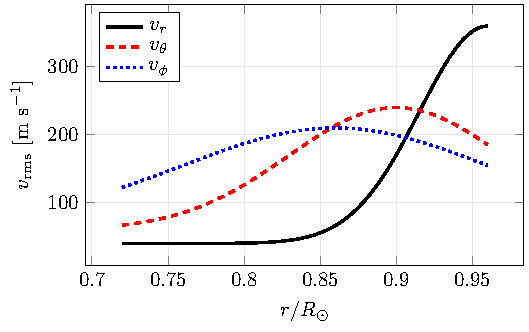
\includegraphics[width=0.7\linewidth]{sample.pdf}
  \caption{図の説明。キャプションだけを読んで何の図か分かるように書くこと。
    軸の量と単位、線や色が何を表すか、どの計算・観測のものかを含める。}
  \label{fig:sample}
\end{figure}

図\ref{fig:sample}に\todo{何を示した図か}を示す。

%% 図を横に並べて (a) (b) と番号を振る例。subcaption パッケージを使う。
\begin{figure}[tb]
  \centering
  \begin{subfigure}{0.48\linewidth}
    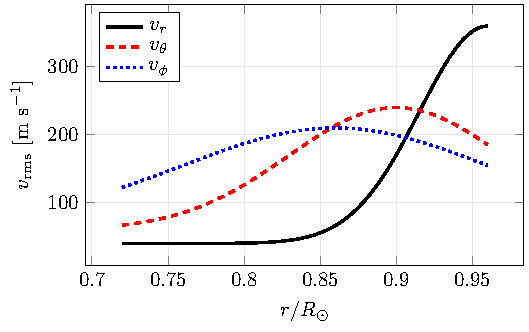
\includegraphics[width=\linewidth]{sample.pdf}
    \caption{低解像度}
    \label{fig:comp_low}
  \end{subfigure}\hfill
  \begin{subfigure}{0.48\linewidth}
    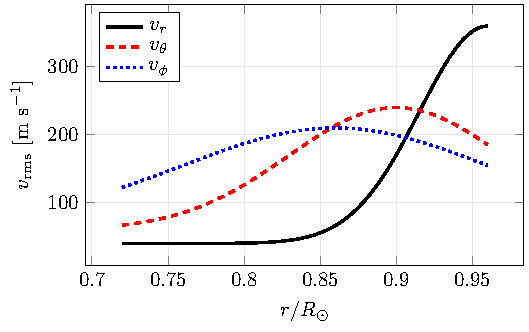
\includegraphics[width=\linewidth]{sample.pdf}
    \caption{高解像度}
    \label{fig:comp_high}
  \end{subfigure}
  \caption{解像度による対流構造の違い。個々の図は
    図\ref{fig:comp_low}、図\ref{fig:comp_high} のように参照できる。}
  \label{fig:comp}
\end{figure}


\chapter{議論}
\label{chap:discussion}

%% 議論の章でやることは 3 つです。
%%   1. 結果の解釈：なぜそうなったのかを物理で説明する
%%   2. 先行研究との比較：一致するのか、しないのか。しないならなぜか
%%   3. 限界：この研究で言えないことは何か
%% 3 を書くのを怖がらないでください。限界を自分で把握できていることは
%% 減点ではなく加点になります。

\section{結果の解釈}
\label{sec:discussion_interpretation}

\todo{書く}

\section{先行研究との比較}
\label{sec:discussion_comparison}

\todo{書く}

\section{本研究の限界}
\label{sec:discussion_limitation}

\todo{書く}


\chapter{結論}
\label{chap:conclusion}

%% 結論は「まとめ」ではなく、序論で立てた問いに対する答えを短く言い切る場所です。
%% 新しい図やデータはここでは出しません。
%% 最後に今後の展望を 1 段落だけ書きます。

本研究では\todo{何をしたか}を行った。その結果、以下のことが分かった。

\begin{enumerate}
  \item \todo{結論 1}
  \item \todo{結論 2}
\end{enumerate}

今後は\todo{展望}が課題である。


%% 執筆の手引き。自分の原稿が形になったら、この行をコメントアウトする。
% !TEX root = main.tex
%% ===========================================================================
%%  執筆の手引き
%%
%%  論文の中身ではなく書き方の説明です。書き始める前に一度目を通してください。
%%  自分の原稿が形になってきたら、main.tex の % !TEX root = main.tex
%% ===========================================================================
%%  執筆の手引き
%%
%%  論文の中身ではなく書き方の説明です。書き始める前に一度目を通してください。
%%  自分の原稿が形になってきたら、main.tex の % !TEX root = main.tex
%% ===========================================================================
%%  執筆の手引き
%%
%%  論文の中身ではなく書き方の説明です。書き始める前に一度目を通してください。
%%  自分の原稿が形になってきたら、main.tex の \input{guide} を
%%  コメントアウトして構いません。
%% ===========================================================================

\chapter{執筆の手引き}
\label{chap:guide}

\section{文章の書き方}

\subsection{論文は主張の連なりである}

修士論文でよくある失敗は、やったことを時系列で並べてしまうことである。
読者が知りたいのは君が何を試したかの記録ではなく、
\textbf{何が新しく分かったのか}と\textbf{なぜそう言えるのか}の二つだけである。
まず結論を決め、その結論を支えるのに必要な材料だけを、必要な順に並べる。
やったが結論に効かなかった作業は、付録に回すか、思い切って落とす。

\subsection{一つの段落には一つの主張}

段落の先頭の一文（トピックセンテンス）にその段落の主張を書き、
残りの文でそれを支える。段落の頭だけを拾い読みして論旨が通るなら、
その章はよく書けている。

\subsection{日本語の作法}

\begin{description}
  \item[主語と述語を近づける] 間に修飾句を挟むほど読みにくくなる。
    一文が 3 行を超えたら、ほぼ確実に切れる。
  \item[「〜と考えられる」を減らす] 自分の結果について書くときは
    「〜である」と言い切る。断定できないなら、なぜ断定できないかを書く。
  \item[主観語を使わない] 「非常に」「かなり」「劇的に」は情報を持たない。
    「3 倍大きい」と書く。
  \item[「思う」は使わない] 論文は感想文ではない。
  \item[用語を統一する] 「対流セル」と「対流構造」を無意識に混ぜない。
    同じものは同じ語で呼び、違うものは違う語で呼ぶ。
  \item[数式も文の一部] 式の前後の助詞をつなげて音読し、
    日本語として成立するか確かめる。
\end{description}

\subsection{単位と有効数字}

物理量には必ず単位をつける。数値の有効数字は測定・計算の精度に見合った桁数にする。
計算機が出した 8 桁をそのまま書き写さない。
単位つきの量は \texttt{siunitx} を使うと組版が揃う。

\begin{verbatim}
太陽半径は \qty{6.96e8}{m}、自転角速度は \qty{2.6e-6}{\per\second} である。
速度は \qty{2}{\km\per\second}、範囲は \qtyrange{1}{5}{\km\per\second}。
\end{verbatim}

\noindent
従来どおり \verb|$2~\mathrm{km~s^{-1}}$| と手で書いてもよいが、
論文全体でどちらかに統一すること。

\subsection{書き始められないとき}

完成形を頭の中で作ってから書こうとすると、いつまでも書き始められない。
図を先に作り、それを並べ替えて話の順番を決め、
各図に対して説明の段落を書く、という順で進めるとよい。
文章の質は推敲で上げるもので、初稿で上げるものではない。


\section{\LaTeX{} の使い方}
\label{sec:guide_latex}

\subsection{このテンプレートの構成}

\begin{description}
  \item[\texttt{main.tex}] プリアンブル、表紙に載る情報、概要、章の並び。
    自分用に書き換えるのは主にこのファイルの上半分である。
  \item[\texttt{body.tex}] 本文。序論から結論まで。
  \item[\texttt{guide.tex}] この手引き。書き終わったら外してよい。
  \item[\texttt{thesis.bib}] 引用文献のデータベース。
  \item[\texttt{achilles.sty}] 全テンプレート共通のプリアンブル。
    原本はリポジトリの \texttt{common/} にある。
  \item[\texttt{thesiscover.sty}] 表紙のレイアウト。通常は触らない。
  \item[\texttt{fig/}] 図を置くところ。
\end{description}

\subsection{コンパイル}

このディレクトリで
\begin{verbatim}
latexmk
\end{verbatim}
とすれば \texttt{main.pdf} ができる。書きながら自動で作り直したいときは
\begin{verbatim}
latexmk -pvc
\end{verbatim}
とする。中間ファイルがおかしくなったら \verb|latexmk -C| で全部消してやり直す。
エンジンは LuaLaTeX である。\texttt{platex} や \texttt{uplatex} では通らない。

\subsection{相互参照}

図・表・式・章には \verb|\label{}| をつけ、本文からは \verb|\ref{}| で参照する。
番号を手で書いてはいけない。あとで章を入れ替えたときに必ず破綻する。
ラベルには \verb|fig:|、\verb|tab:|、\verb|eq:|、\verb|sec:|、\verb|chap:| の
接頭辞をつけると、何を指しているか分かりやすい。

\begin{verbatim}
図\ref{fig:sample}に示すように……
式\eqref{eq:induction}より……
\end{verbatim}

\noindent
式の参照は \verb|\ref| ではなく \verb|\eqref| を使うと括弧がつく。

\subsection{引用}

\texttt{thesis.bib} に文献情報を書き、本文から \verb|\citep| か \verb|\citet| で引く。
NASA ADS の \textsf{Export Citation} から \textsf{BibTeX} を選べば、
そのまま貼り付けられる形式で得られる。手で打ち直さないこと。

\begin{verbatim}
小スケールダイナモが有効粘性を下げる \citep{hotta2021}。
\citet{hotta2021} はこれを高解像度計算で示した。
\end{verbatim}

\noindent
このテンプレートは \texttt{biblatex + biber} と \texttt{natbib + bst} の
どちらでも動くようにしてある。\texttt{main.tex} の冒頭で切り替える。
本文の書き方は両者で共通なので、あとから変えても原稿は書き直さなくてよい。

\subsection{数式}

番号をつけて後で参照する式は \texttt{align}、参照しない式は \texttt{align*} を使う。
\verb|$$ ... $$| は使わない（\LaTeX{} では非推奨で、前後の空きがおかしくなる）。
ベクトルは \verb|\vect{B}| と書くと太字斜体になる。
\verb|\grad|、\verb|\divergence|、\verb|\curl|、\verb|\pdif{}{}| などの
短縮マクロを \texttt{achilles.sty} に用意してある。

\subsection{よくあるつまずき}

\begin{description}
  \item[エラーが出たら一番上から読む] 後ろのエラーは前のエラーの巻き添えである
    ことが多い。\verb|! LaTeX Error:| で始まる最初の行と、その直前の行番号を見る。
  \item[Undefined control sequence] マクロの綴りが違うか、
    必要なパッケージを読み込んでいない。
  \item[Overfull \textbackslash hbox] 行がはみ出している。長い英単語や URL が原因。
    数 pt なら無視してよいが、目で見て飛び出していたら直す。
  \item[番号が \texttt{??} になる] 参照が解決していない。もう一度コンパイルする
    （\texttt{latexmk} なら自動でやる）。それでも直らないならラベルの綴り間違い。
  \item[図が出ない] ファイル名か拡張子が違う。LuaLaTeX が読めるのは
    PDF・PNG・JPEG である。EPS は事前に PDF へ変換しておく。
\end{description}


\section{図表の作り方}
\label{sec:guide_figure}

審査員は本文より先に図を見る。図が分かりやすければ論文は半分伝わったも同然である。
逆に、図が読めない論文は本文がどれだけ良くても評価されない。

\subsection{形式}

\begin{description}
  \item[線画はベクタ形式で] 折れ線・等高線・散布図は PDF で保存する。
    拡大しても線が滑らかで、印刷しても綺麗である。
    Matplotlib なら \verb|plt.savefig('foo.pdf')| とするだけである。
  \item[画像はラスタ形式で] 太陽表面の強度分布のような画素の塊は PNG にする。
    PDF にすると数十 MB になり、PDF ビューアが固まる。
    \verb|dpi=300| 程度あれば印刷に耐える。
  \item[JPEG は使わない] 圧縮による滲みが出る。写真以外では使わない。
\end{description}

\subsection{文字の大きさ}

図の中の文字が本文より小さいと読めない。
論文に貼ったときに\textbf{本文と同じかやや小さい程度}になるよう、
図を作る段階でフォントサイズを決める。
\verb|\includegraphics[width=0.5\linewidth]| のように後から縮めると
文字も一緒に縮むので、その分を見越しておく。
出来上がった PDF を 100\% 表示にして、読めるか自分の目で確かめること。

\subsection{色}

\begin{description}
  \item[虹色（jet）を使わない] 明度が単調でないため、
    データにない偽の構造が見えてしまう。Matplotlib の既定である
    \texttt{viridis} や、正負のある量には \texttt{RdBu\_r} のような
    発散型カラーマップを使う。
  \item[色覚多様性に配慮する] 日本人男性の約 5\% は赤と緑の区別がつきにくい。
    赤と緑だけで系列を区別しない。線種（実線・破線・点線）や
    マーカーの形も併せて変える。
  \item[白黒で印刷されても読めるか] 製本された論文が白黒コピーされることはある。
    色を消しても情報が失われないようにしておくと安全である。
  \item[色に意味を持たせたら統一する] 論文全体で「観測は黒、計算は赤」と決めたら、
    最後まで変えない。
\end{description}

\subsection{キャプション}

キャプションだけを読んで図が理解できるように書く。含めるべきものは
\begin{enumerate}
  \item 何を示した図か
  \item 軸の量と単位
  \item 線・色・記号がそれぞれ何を表すか
  \item どの計算・観測のデータか
\end{enumerate}
である。「結果」だけのキャプションは論外である。
図のキャプションは図の\textbf{下}、表のキャプションは表の\textbf{上}に置く。

\subsection{図を並べる}

\texttt{subcaption} パッケージで (a) (b) と番号を振れる。

\begin{verbatim}
\begin{figure}[tb]
  \centering
  \begin{subfigure}{0.48\linewidth}
    \includegraphics[width=\linewidth]{left.pdf}
    \caption{低解像度}\label{fig:comp_low}
  \end{subfigure}\hfill
  \begin{subfigure}{0.48\linewidth}
    \includegraphics[width=\linewidth]{right.pdf}
    \caption{高解像度}\label{fig:comp_high}
  \end{subfigure}
  \caption{解像度による対流構造の違い。}
  \label{fig:comp}
\end{figure}
\end{verbatim}

\subsection{図の位置が思いどおりにならないとき}

\LaTeX{} は図を「浮きもの」として扱い、ページの切れ目を見て適当な場所に置く。
\verb|[tb]| は「ページの上か下に置いてよい」という指定である。
\verb|[h]|（ここに置け）を多用すると、かえって図が後ろに溜まる。
最終稿になるまでは位置を気にせず、内容を書くことに集中したほうがよい。


\section{引用と剽窃}
\label{sec:guide_ethics}

これは作法の問題ではなく、研究者としての資格の問題である。
剽窃が発覚すれば学位は取り消される。指導教員にも累が及ぶ。
知らなかったでは済まないので、必ず読むこと。

\subsection{何が剽窃か}

他人の文章・図・アイデアを、出典を示さずに自分のものとして提示することは
すべて剽窃である。以下はいずれも剽窃にあたる。

\begin{itemize}
  \item 論文や web の文章をコピーして貼り、少し語尾を変えて自分の文にする
  \item 他人の図をキャプションに出典を書かずに載せる
  \item 先輩の修士論文から章をまるごと持ってくる
  \item 生成 AI が出力した文章を、出典も検証もなくそのまま載せる
  \item 自分の過去の論文から、断りなく文章を再利用する（自己剽窃）
\end{itemize}

\subsection{正しいやり方}

\begin{description}
  \item[事実や知見を借りるとき] 自分の言葉で書き直し、引用をつける。
    「対流層の底は $0.71\,R_\odot$ にある \citep{christensen-dalsgaard1991}。」
  \item[文章をそのまま使うとき] 引用符でくくり、出典を示す。
    ただし自然科学の論文で原文引用が必要になることはまずない。
    必要だと思ったら、たいていは自分の言葉で書き直すべき場面である。
  \item[図を借りるとき] キャプションの末尾に出典を書く。
    「\citet{hotta2021} の Figure 3 を改変。」
    商業出版社の論文図は、多くの場合、著者本人でも転載に許諾が要る。
    論文の web ページにある \textsf{Permissions} や \textsf{RightsLink} から
    手続きする。許諾が取れないなら、自分で描き直す。
\end{description}

\noindent
どこまで自分の言葉にすればよいかの基準は、
語順を入れ替えたか同義語に置き換えたかではない。
\textbf{元の文章を見ずに、理解した内容を自分で書けるか}である。
見ないと書けないなら、まだ理解していない。

\subsection{生成 AI の扱い}

英文の校正や、書き出しに詰まったときの相談に使うのは構わない。
ただし次の 3 点は守ること。

\begin{enumerate}
  \item 出力された内容の正しさは自分で確認する。
    存在しない論文を引用してくることがある。
  \item 引用文献は必ず ADS などの一次情報で実在を確かめる。
  \item 使い方について、指導教員に隠さない。
    大学や学会が定める方針にも従うこと。
\end{enumerate}

\noindent
自分が説明できない文章を論文に載せてはいけない。
審査で問われるのは論文ではなく、書いた本人だからである。

\subsection{データと図の加工}

都合の悪い点を消す、エラーバーを小さく見せる、
軸を切って差を大きく見せる、といった操作は捏造・改竄である。
処理を加えたなら、加えたことを本文に書く。
「見やすさのために平滑化した」と書けば済む話を、黙ってやると不正になる。


\section{原稿の管理と添削の受け方}
\label{sec:guide_review}

\subsection{Git で履歴を残す}

\texttt{.tex} はテキストファイルなので Git で管理できる。
締切前に「昨日の版に戻したい」と言い出す前に、最初から履歴を残しておくこと。
節を書き終えるたび、あるいは一日の終わりに
\begin{verbatim}
git add -A
git commit -m "序論の先行研究を追加"
\end{verbatim}
としておけばよい。中間ファイルや PDF は \texttt{.gitignore} で除外してある。
バックアップは Git だけに頼らず、クラウド（大学のストレージなど）にも置くこと。

\subsection{添削に出す前に自分でやること}

指導教員の時間を、自分で見つけられる誤りに使わせないこと。
出す前に次を済ませておく。

\begin{itemize}
  \item \verb|\todo| と \verb|\red| が残っていないか検索する
  \item \texttt{??} や \texttt{[?]} が PDF に出ていないか確認する
  \item 図がすべて本文から参照されているか確認する
  \item 通しで一度、声に出して読む（黙読よりずっと効く。文の切れ目が分かる）
  \item 数式の記号がすべて本文で定義されているか確認する
\end{itemize}

\subsection{添削の受け方}

\begin{description}
  \item[早く出す] 完璧になってから見せようとすると間に合わない。
    構成だけの段階、章ごと、と何度も出したほうが結果的に速い。
  \item[版に名前をつける] PDF は \texttt{thesis\_20270105.pdf} のように
    日付をつけて渡す。「最新版」が何を指すか分からなくなるのを防ぐ。
  \item[指摘の理由を理解する] 直せと言われた箇所だけ直すと、
    同じ誤りを他の場所に残したまま次の版を出すことになる。
    なぜそう指摘されたのかを考え、同種の箇所をまとめて直す。
  \item[納得できないときは聞く] 指摘が間違っていることもある。
    黙って従うのも、黙って無視するのも良くない。
  \item[直したかどうかを返す] どの指摘をどう直したか、
    直さなかったならなぜかを添えて返すと、次の添削が速くなる。
\end{description}

\subsection{変更点を見せる}

\texttt{latexdiff} を使うと、前の版からの変更箇所に下線と取り消し線がついた
PDF を作れる。どこを直したかが一目で分かるので、
再添削のときはこれを添えると親切である。

\begin{verbatim}
latexdiff-vc --git -r HEAD~1 --flatten main.tex
\end{verbatim}

\subsection{提出前の最終確認}

\begin{itemize}
  \item 表紙の年度・題目・氏名・学籍番号・所属が学務の書類と一致しているか
  \item ページ番号が通っているか
  \item 目次・図目次・表目次の番号が本文と合っているか
  \item 引用文献が本文の引用とすべて対応しているか
  \item 手引き（この章）を \texttt{main.tex} から外したか
  \item 行番号（\texttt{lineno}）を切ったか
  \item 印刷して提出するなら、リンクの色を黒にしたか
  \item PDF を実際に印刷して、図の文字が読めるか確かめたか
\end{itemize}
 を
%%  コメントアウトして構いません。
%% ===========================================================================

\chapter{執筆の手引き}
\label{chap:guide}

\section{文章の書き方}

\subsection{論文は主張の連なりである}

修士論文でよくある失敗は、やったことを時系列で並べてしまうことである。
読者が知りたいのは君が何を試したかの記録ではなく、
\textbf{何が新しく分かったのか}と\textbf{なぜそう言えるのか}の二つだけである。
まず結論を決め、その結論を支えるのに必要な材料だけを、必要な順に並べる。
やったが結論に効かなかった作業は、付録に回すか、思い切って落とす。

\subsection{一つの段落には一つの主張}

段落の先頭の一文（トピックセンテンス）にその段落の主張を書き、
残りの文でそれを支える。段落の頭だけを拾い読みして論旨が通るなら、
その章はよく書けている。

\subsection{日本語の作法}

\begin{description}
  \item[主語と述語を近づける] 間に修飾句を挟むほど読みにくくなる。
    一文が 3 行を超えたら、ほぼ確実に切れる。
  \item[「〜と考えられる」を減らす] 自分の結果について書くときは
    「〜である」と言い切る。断定できないなら、なぜ断定できないかを書く。
  \item[主観語を使わない] 「非常に」「かなり」「劇的に」は情報を持たない。
    「3 倍大きい」と書く。
  \item[「思う」は使わない] 論文は感想文ではない。
  \item[用語を統一する] 「対流セル」と「対流構造」を無意識に混ぜない。
    同じものは同じ語で呼び、違うものは違う語で呼ぶ。
  \item[数式も文の一部] 式の前後の助詞をつなげて音読し、
    日本語として成立するか確かめる。
\end{description}

\subsection{単位と有効数字}

物理量には必ず単位をつける。数値の有効数字は測定・計算の精度に見合った桁数にする。
計算機が出した 8 桁をそのまま書き写さない。
単位つきの量は \texttt{siunitx} を使うと組版が揃う。

\begin{verbatim}
太陽半径は \qty{6.96e8}{m}、自転角速度は \qty{2.6e-6}{\per\second} である。
速度は \qty{2}{\km\per\second}、範囲は \qtyrange{1}{5}{\km\per\second}。
\end{verbatim}

\noindent
従来どおり \verb|$2~\mathrm{km~s^{-1}}$| と手で書いてもよいが、
論文全体でどちらかに統一すること。

\subsection{書き始められないとき}

完成形を頭の中で作ってから書こうとすると、いつまでも書き始められない。
図を先に作り、それを並べ替えて話の順番を決め、
各図に対して説明の段落を書く、という順で進めるとよい。
文章の質は推敲で上げるもので、初稿で上げるものではない。


\section{\LaTeX{} の使い方}
\label{sec:guide_latex}

\subsection{このテンプレートの構成}

\begin{description}
  \item[\texttt{main.tex}] プリアンブル、表紙に載る情報、概要、章の並び。
    自分用に書き換えるのは主にこのファイルの上半分である。
  \item[\texttt{body.tex}] 本文。序論から結論まで。
  \item[\texttt{guide.tex}] この手引き。書き終わったら外してよい。
  \item[\texttt{thesis.bib}] 引用文献のデータベース。
  \item[\texttt{achilles.sty}] 全テンプレート共通のプリアンブル。
    原本はリポジトリの \texttt{common/} にある。
  \item[\texttt{thesiscover.sty}] 表紙のレイアウト。通常は触らない。
  \item[\texttt{fig/}] 図を置くところ。
\end{description}

\subsection{コンパイル}

このディレクトリで
\begin{verbatim}
latexmk
\end{verbatim}
とすれば \texttt{main.pdf} ができる。書きながら自動で作り直したいときは
\begin{verbatim}
latexmk -pvc
\end{verbatim}
とする。中間ファイルがおかしくなったら \verb|latexmk -C| で全部消してやり直す。
エンジンは LuaLaTeX である。\texttt{platex} や \texttt{uplatex} では通らない。

\subsection{相互参照}

図・表・式・章には \verb|\label{}| をつけ、本文からは \verb|\ref{}| で参照する。
番号を手で書いてはいけない。あとで章を入れ替えたときに必ず破綻する。
ラベルには \verb|fig:|、\verb|tab:|、\verb|eq:|、\verb|sec:|、\verb|chap:| の
接頭辞をつけると、何を指しているか分かりやすい。

\begin{verbatim}
図\ref{fig:sample}に示すように……
式\eqref{eq:induction}より……
\end{verbatim}

\noindent
式の参照は \verb|\ref| ではなく \verb|\eqref| を使うと括弧がつく。

\subsection{引用}

\texttt{thesis.bib} に文献情報を書き、本文から \verb|\citep| か \verb|\citet| で引く。
NASA ADS の \textsf{Export Citation} から \textsf{BibTeX} を選べば、
そのまま貼り付けられる形式で得られる。手で打ち直さないこと。

\begin{verbatim}
小スケールダイナモが有効粘性を下げる \citep{hotta2021}。
\citet{hotta2021} はこれを高解像度計算で示した。
\end{verbatim}

\noindent
このテンプレートは \texttt{biblatex + biber} と \texttt{natbib + bst} の
どちらでも動くようにしてある。\texttt{main.tex} の冒頭で切り替える。
本文の書き方は両者で共通なので、あとから変えても原稿は書き直さなくてよい。

\subsection{数式}

番号をつけて後で参照する式は \texttt{align}、参照しない式は \texttt{align*} を使う。
\verb|$$ ... $$| は使わない（\LaTeX{} では非推奨で、前後の空きがおかしくなる）。
ベクトルは \verb|\vect{B}| と書くと太字斜体になる。
\verb|\grad|、\verb|\divergence|、\verb|\curl|、\verb|\pdif{}{}| などの
短縮マクロを \texttt{achilles.sty} に用意してある。

\subsection{よくあるつまずき}

\begin{description}
  \item[エラーが出たら一番上から読む] 後ろのエラーは前のエラーの巻き添えである
    ことが多い。\verb|! LaTeX Error:| で始まる最初の行と、その直前の行番号を見る。
  \item[Undefined control sequence] マクロの綴りが違うか、
    必要なパッケージを読み込んでいない。
  \item[Overfull \textbackslash hbox] 行がはみ出している。長い英単語や URL が原因。
    数 pt なら無視してよいが、目で見て飛び出していたら直す。
  \item[番号が \texttt{??} になる] 参照が解決していない。もう一度コンパイルする
    （\texttt{latexmk} なら自動でやる）。それでも直らないならラベルの綴り間違い。
  \item[図が出ない] ファイル名か拡張子が違う。LuaLaTeX が読めるのは
    PDF・PNG・JPEG である。EPS は事前に PDF へ変換しておく。
\end{description}


\section{図表の作り方}
\label{sec:guide_figure}

審査員は本文より先に図を見る。図が分かりやすければ論文は半分伝わったも同然である。
逆に、図が読めない論文は本文がどれだけ良くても評価されない。

\subsection{形式}

\begin{description}
  \item[線画はベクタ形式で] 折れ線・等高線・散布図は PDF で保存する。
    拡大しても線が滑らかで、印刷しても綺麗である。
    Matplotlib なら \verb|plt.savefig('foo.pdf')| とするだけである。
  \item[画像はラスタ形式で] 太陽表面の強度分布のような画素の塊は PNG にする。
    PDF にすると数十 MB になり、PDF ビューアが固まる。
    \verb|dpi=300| 程度あれば印刷に耐える。
  \item[JPEG は使わない] 圧縮による滲みが出る。写真以外では使わない。
\end{description}

\subsection{文字の大きさ}

図の中の文字が本文より小さいと読めない。
論文に貼ったときに\textbf{本文と同じかやや小さい程度}になるよう、
図を作る段階でフォントサイズを決める。
\verb|\includegraphics[width=0.5\linewidth]| のように後から縮めると
文字も一緒に縮むので、その分を見越しておく。
出来上がった PDF を 100\% 表示にして、読めるか自分の目で確かめること。

\subsection{色}

\begin{description}
  \item[虹色（jet）を使わない] 明度が単調でないため、
    データにない偽の構造が見えてしまう。Matplotlib の既定である
    \texttt{viridis} や、正負のある量には \texttt{RdBu\_r} のような
    発散型カラーマップを使う。
  \item[色覚多様性に配慮する] 日本人男性の約 5\% は赤と緑の区別がつきにくい。
    赤と緑だけで系列を区別しない。線種（実線・破線・点線）や
    マーカーの形も併せて変える。
  \item[白黒で印刷されても読めるか] 製本された論文が白黒コピーされることはある。
    色を消しても情報が失われないようにしておくと安全である。
  \item[色に意味を持たせたら統一する] 論文全体で「観測は黒、計算は赤」と決めたら、
    最後まで変えない。
\end{description}

\subsection{キャプション}

キャプションだけを読んで図が理解できるように書く。含めるべきものは
\begin{enumerate}
  \item 何を示した図か
  \item 軸の量と単位
  \item 線・色・記号がそれぞれ何を表すか
  \item どの計算・観測のデータか
\end{enumerate}
である。「結果」だけのキャプションは論外である。
図のキャプションは図の\textbf{下}、表のキャプションは表の\textbf{上}に置く。

\subsection{図を並べる}

\texttt{subcaption} パッケージで (a) (b) と番号を振れる。

\begin{verbatim}
\begin{figure}[tb]
  \centering
  \begin{subfigure}{0.48\linewidth}
    \includegraphics[width=\linewidth]{left.pdf}
    \caption{低解像度}\label{fig:comp_low}
  \end{subfigure}\hfill
  \begin{subfigure}{0.48\linewidth}
    \includegraphics[width=\linewidth]{right.pdf}
    \caption{高解像度}\label{fig:comp_high}
  \end{subfigure}
  \caption{解像度による対流構造の違い。}
  \label{fig:comp}
\end{figure}
\end{verbatim}

\subsection{図の位置が思いどおりにならないとき}

\LaTeX{} は図を「浮きもの」として扱い、ページの切れ目を見て適当な場所に置く。
\verb|[tb]| は「ページの上か下に置いてよい」という指定である。
\verb|[h]|（ここに置け）を多用すると、かえって図が後ろに溜まる。
最終稿になるまでは位置を気にせず、内容を書くことに集中したほうがよい。


\section{引用と剽窃}
\label{sec:guide_ethics}

これは作法の問題ではなく、研究者としての資格の問題である。
剽窃が発覚すれば学位は取り消される。指導教員にも累が及ぶ。
知らなかったでは済まないので、必ず読むこと。

\subsection{何が剽窃か}

他人の文章・図・アイデアを、出典を示さずに自分のものとして提示することは
すべて剽窃である。以下はいずれも剽窃にあたる。

\begin{itemize}
  \item 論文や web の文章をコピーして貼り、少し語尾を変えて自分の文にする
  \item 他人の図をキャプションに出典を書かずに載せる
  \item 先輩の修士論文から章をまるごと持ってくる
  \item 生成 AI が出力した文章を、出典も検証もなくそのまま載せる
  \item 自分の過去の論文から、断りなく文章を再利用する（自己剽窃）
\end{itemize}

\subsection{正しいやり方}

\begin{description}
  \item[事実や知見を借りるとき] 自分の言葉で書き直し、引用をつける。
    「対流層の底は $0.71\,R_\odot$ にある \citep{christensen-dalsgaard1991}。」
  \item[文章をそのまま使うとき] 引用符でくくり、出典を示す。
    ただし自然科学の論文で原文引用が必要になることはまずない。
    必要だと思ったら、たいていは自分の言葉で書き直すべき場面である。
  \item[図を借りるとき] キャプションの末尾に出典を書く。
    「\citet{hotta2021} の Figure 3 を改変。」
    商業出版社の論文図は、多くの場合、著者本人でも転載に許諾が要る。
    論文の web ページにある \textsf{Permissions} や \textsf{RightsLink} から
    手続きする。許諾が取れないなら、自分で描き直す。
\end{description}

\noindent
どこまで自分の言葉にすればよいかの基準は、
語順を入れ替えたか同義語に置き換えたかではない。
\textbf{元の文章を見ずに、理解した内容を自分で書けるか}である。
見ないと書けないなら、まだ理解していない。

\subsection{生成 AI の扱い}

英文の校正や、書き出しに詰まったときの相談に使うのは構わない。
ただし次の 3 点は守ること。

\begin{enumerate}
  \item 出力された内容の正しさは自分で確認する。
    存在しない論文を引用してくることがある。
  \item 引用文献は必ず ADS などの一次情報で実在を確かめる。
  \item 使い方について、指導教員に隠さない。
    大学や学会が定める方針にも従うこと。
\end{enumerate}

\noindent
自分が説明できない文章を論文に載せてはいけない。
審査で問われるのは論文ではなく、書いた本人だからである。

\subsection{データと図の加工}

都合の悪い点を消す、エラーバーを小さく見せる、
軸を切って差を大きく見せる、といった操作は捏造・改竄である。
処理を加えたなら、加えたことを本文に書く。
「見やすさのために平滑化した」と書けば済む話を、黙ってやると不正になる。


\section{原稿の管理と添削の受け方}
\label{sec:guide_review}

\subsection{Git で履歴を残す}

\texttt{.tex} はテキストファイルなので Git で管理できる。
締切前に「昨日の版に戻したい」と言い出す前に、最初から履歴を残しておくこと。
節を書き終えるたび、あるいは一日の終わりに
\begin{verbatim}
git add -A
git commit -m "序論の先行研究を追加"
\end{verbatim}
としておけばよい。中間ファイルや PDF は \texttt{.gitignore} で除外してある。
バックアップは Git だけに頼らず、クラウド（大学のストレージなど）にも置くこと。

\subsection{添削に出す前に自分でやること}

指導教員の時間を、自分で見つけられる誤りに使わせないこと。
出す前に次を済ませておく。

\begin{itemize}
  \item \verb|\todo| と \verb|\red| が残っていないか検索する
  \item \texttt{??} や \texttt{[?]} が PDF に出ていないか確認する
  \item 図がすべて本文から参照されているか確認する
  \item 通しで一度、声に出して読む（黙読よりずっと効く。文の切れ目が分かる）
  \item 数式の記号がすべて本文で定義されているか確認する
\end{itemize}

\subsection{添削の受け方}

\begin{description}
  \item[早く出す] 完璧になってから見せようとすると間に合わない。
    構成だけの段階、章ごと、と何度も出したほうが結果的に速い。
  \item[版に名前をつける] PDF は \texttt{thesis\_20270105.pdf} のように
    日付をつけて渡す。「最新版」が何を指すか分からなくなるのを防ぐ。
  \item[指摘の理由を理解する] 直せと言われた箇所だけ直すと、
    同じ誤りを他の場所に残したまま次の版を出すことになる。
    なぜそう指摘されたのかを考え、同種の箇所をまとめて直す。
  \item[納得できないときは聞く] 指摘が間違っていることもある。
    黙って従うのも、黙って無視するのも良くない。
  \item[直したかどうかを返す] どの指摘をどう直したか、
    直さなかったならなぜかを添えて返すと、次の添削が速くなる。
\end{description}

\subsection{変更点を見せる}

\texttt{latexdiff} を使うと、前の版からの変更箇所に下線と取り消し線がついた
PDF を作れる。どこを直したかが一目で分かるので、
再添削のときはこれを添えると親切である。

\begin{verbatim}
latexdiff-vc --git -r HEAD~1 --flatten main.tex
\end{verbatim}

\subsection{提出前の最終確認}

\begin{itemize}
  \item 表紙の年度・題目・氏名・学籍番号・所属が学務の書類と一致しているか
  \item ページ番号が通っているか
  \item 目次・図目次・表目次の番号が本文と合っているか
  \item 引用文献が本文の引用とすべて対応しているか
  \item 手引き（この章）を \texttt{main.tex} から外したか
  \item 行番号（\texttt{lineno}）を切ったか
  \item 印刷して提出するなら、リンクの色を黒にしたか
  \item PDF を実際に印刷して、図の文字が読めるか確かめたか
\end{itemize}
 を
%%  コメントアウトして構いません。
%% ===========================================================================

\chapter{執筆の手引き}
\label{chap:guide}

\section{文章の書き方}

\subsection{論文は主張の連なりである}

修士論文でよくある失敗は、やったことを時系列で並べてしまうことである。
読者が知りたいのは君が何を試したかの記録ではなく、
\textbf{何が新しく分かったのか}と\textbf{なぜそう言えるのか}の二つだけである。
まず結論を決め、その結論を支えるのに必要な材料だけを、必要な順に並べる。
やったが結論に効かなかった作業は、付録に回すか、思い切って落とす。

\subsection{一つの段落には一つの主張}

段落の先頭の一文（トピックセンテンス）にその段落の主張を書き、
残りの文でそれを支える。段落の頭だけを拾い読みして論旨が通るなら、
その章はよく書けている。

\subsection{日本語の作法}

\begin{description}
  \item[主語と述語を近づける] 間に修飾句を挟むほど読みにくくなる。
    一文が 3 行を超えたら、ほぼ確実に切れる。
  \item[「〜と考えられる」を減らす] 自分の結果について書くときは
    「〜である」と言い切る。断定できないなら、なぜ断定できないかを書く。
  \item[主観語を使わない] 「非常に」「かなり」「劇的に」は情報を持たない。
    「3 倍大きい」と書く。
  \item[「思う」は使わない] 論文は感想文ではない。
  \item[用語を統一する] 「対流セル」と「対流構造」を無意識に混ぜない。
    同じものは同じ語で呼び、違うものは違う語で呼ぶ。
  \item[数式も文の一部] 式の前後の助詞をつなげて音読し、
    日本語として成立するか確かめる。
\end{description}

\subsection{単位と有効数字}

物理量には必ず単位をつける。数値の有効数字は測定・計算の精度に見合った桁数にする。
計算機が出した 8 桁をそのまま書き写さない。
単位つきの量は \texttt{siunitx} を使うと組版が揃う。

\begin{verbatim}
太陽半径は \qty{6.96e8}{m}、自転角速度は \qty{2.6e-6}{\per\second} である。
速度は \qty{2}{\km\per\second}、範囲は \qtyrange{1}{5}{\km\per\second}。
\end{verbatim}

\noindent
従来どおり \verb|$2~\mathrm{km~s^{-1}}$| と手で書いてもよいが、
論文全体でどちらかに統一すること。

\subsection{書き始められないとき}

完成形を頭の中で作ってから書こうとすると、いつまでも書き始められない。
図を先に作り、それを並べ替えて話の順番を決め、
各図に対して説明の段落を書く、という順で進めるとよい。
文章の質は推敲で上げるもので、初稿で上げるものではない。


\section{\LaTeX{} の使い方}
\label{sec:guide_latex}

\subsection{このテンプレートの構成}

\begin{description}
  \item[\texttt{main.tex}] プリアンブル、表紙に載る情報、概要、章の並び。
    自分用に書き換えるのは主にこのファイルの上半分である。
  \item[\texttt{body.tex}] 本文。序論から結論まで。
  \item[\texttt{guide.tex}] この手引き。書き終わったら外してよい。
  \item[\texttt{thesis.bib}] 引用文献のデータベース。
  \item[\texttt{achilles.sty}] 全テンプレート共通のプリアンブル。
    原本はリポジトリの \texttt{common/} にある。
  \item[\texttt{thesiscover.sty}] 表紙のレイアウト。通常は触らない。
  \item[\texttt{fig/}] 図を置くところ。
\end{description}

\subsection{コンパイル}

このディレクトリで
\begin{verbatim}
latexmk
\end{verbatim}
とすれば \texttt{main.pdf} ができる。書きながら自動で作り直したいときは
\begin{verbatim}
latexmk -pvc
\end{verbatim}
とする。中間ファイルがおかしくなったら \verb|latexmk -C| で全部消してやり直す。
エンジンは LuaLaTeX である。\texttt{platex} や \texttt{uplatex} では通らない。

\subsection{相互参照}

図・表・式・章には \verb|\label{}| をつけ、本文からは \verb|\ref{}| で参照する。
番号を手で書いてはいけない。あとで章を入れ替えたときに必ず破綻する。
ラベルには \verb|fig:|、\verb|tab:|、\verb|eq:|、\verb|sec:|、\verb|chap:| の
接頭辞をつけると、何を指しているか分かりやすい。

\begin{verbatim}
図\ref{fig:sample}に示すように……
式\eqref{eq:induction}より……
\end{verbatim}

\noindent
式の参照は \verb|\ref| ではなく \verb|\eqref| を使うと括弧がつく。

\subsection{引用}

\texttt{thesis.bib} に文献情報を書き、本文から \verb|\citep| か \verb|\citet| で引く。
NASA ADS の \textsf{Export Citation} から \textsf{BibTeX} を選べば、
そのまま貼り付けられる形式で得られる。手で打ち直さないこと。

\begin{verbatim}
小スケールダイナモが有効粘性を下げる \citep{hotta2021}。
\citet{hotta2021} はこれを高解像度計算で示した。
\end{verbatim}

\noindent
このテンプレートは \texttt{biblatex + biber} と \texttt{natbib + bst} の
どちらでも動くようにしてある。\texttt{main.tex} の冒頭で切り替える。
本文の書き方は両者で共通なので、あとから変えても原稿は書き直さなくてよい。

\subsection{数式}

番号をつけて後で参照する式は \texttt{align}、参照しない式は \texttt{align*} を使う。
\verb|$$ ... $$| は使わない（\LaTeX{} では非推奨で、前後の空きがおかしくなる）。
ベクトルは \verb|\vect{B}| と書くと太字斜体になる。
\verb|\grad|、\verb|\divergence|、\verb|\curl|、\verb|\pdif{}{}| などの
短縮マクロを \texttt{achilles.sty} に用意してある。

\subsection{よくあるつまずき}

\begin{description}
  \item[エラーが出たら一番上から読む] 後ろのエラーは前のエラーの巻き添えである
    ことが多い。\verb|! LaTeX Error:| で始まる最初の行と、その直前の行番号を見る。
  \item[Undefined control sequence] マクロの綴りが違うか、
    必要なパッケージを読み込んでいない。
  \item[Overfull \textbackslash hbox] 行がはみ出している。長い英単語や URL が原因。
    数 pt なら無視してよいが、目で見て飛び出していたら直す。
  \item[番号が \texttt{??} になる] 参照が解決していない。もう一度コンパイルする
    （\texttt{latexmk} なら自動でやる）。それでも直らないならラベルの綴り間違い。
  \item[図が出ない] ファイル名か拡張子が違う。LuaLaTeX が読めるのは
    PDF・PNG・JPEG である。EPS は事前に PDF へ変換しておく。
\end{description}


\section{図表の作り方}
\label{sec:guide_figure}

審査員は本文より先に図を見る。図が分かりやすければ論文は半分伝わったも同然である。
逆に、図が読めない論文は本文がどれだけ良くても評価されない。

\subsection{形式}

\begin{description}
  \item[線画はベクタ形式で] 折れ線・等高線・散布図は PDF で保存する。
    拡大しても線が滑らかで、印刷しても綺麗である。
    Matplotlib なら \verb|plt.savefig('foo.pdf')| とするだけである。
  \item[画像はラスタ形式で] 太陽表面の強度分布のような画素の塊は PNG にする。
    PDF にすると数十 MB になり、PDF ビューアが固まる。
    \verb|dpi=300| 程度あれば印刷に耐える。
  \item[JPEG は使わない] 圧縮による滲みが出る。写真以外では使わない。
\end{description}

\subsection{文字の大きさ}

図の中の文字が本文より小さいと読めない。
論文に貼ったときに\textbf{本文と同じかやや小さい程度}になるよう、
図を作る段階でフォントサイズを決める。
\verb|\includegraphics[width=0.5\linewidth]| のように後から縮めると
文字も一緒に縮むので、その分を見越しておく。
出来上がった PDF を 100\% 表示にして、読めるか自分の目で確かめること。

\subsection{色}

\begin{description}
  \item[虹色（jet）を使わない] 明度が単調でないため、
    データにない偽の構造が見えてしまう。Matplotlib の既定である
    \texttt{viridis} や、正負のある量には \texttt{RdBu\_r} のような
    発散型カラーマップを使う。
  \item[色覚多様性に配慮する] 日本人男性の約 5\% は赤と緑の区別がつきにくい。
    赤と緑だけで系列を区別しない。線種（実線・破線・点線）や
    マーカーの形も併せて変える。
  \item[白黒で印刷されても読めるか] 製本された論文が白黒コピーされることはある。
    色を消しても情報が失われないようにしておくと安全である。
  \item[色に意味を持たせたら統一する] 論文全体で「観測は黒、計算は赤」と決めたら、
    最後まで変えない。
\end{description}

\subsection{キャプション}

キャプションだけを読んで図が理解できるように書く。含めるべきものは
\begin{enumerate}
  \item 何を示した図か
  \item 軸の量と単位
  \item 線・色・記号がそれぞれ何を表すか
  \item どの計算・観測のデータか
\end{enumerate}
である。「結果」だけのキャプションは論外である。
図のキャプションは図の\textbf{下}、表のキャプションは表の\textbf{上}に置く。

\subsection{図を並べる}

\texttt{subcaption} パッケージで (a) (b) と番号を振れる。

\begin{verbatim}
\begin{figure}[tb]
  \centering
  \begin{subfigure}{0.48\linewidth}
    \includegraphics[width=\linewidth]{left.pdf}
    \caption{低解像度}\label{fig:comp_low}
  \end{subfigure}\hfill
  \begin{subfigure}{0.48\linewidth}
    \includegraphics[width=\linewidth]{right.pdf}
    \caption{高解像度}\label{fig:comp_high}
  \end{subfigure}
  \caption{解像度による対流構造の違い。}
  \label{fig:comp}
\end{figure}
\end{verbatim}

\subsection{図の位置が思いどおりにならないとき}

\LaTeX{} は図を「浮きもの」として扱い、ページの切れ目を見て適当な場所に置く。
\verb|[tb]| は「ページの上か下に置いてよい」という指定である。
\verb|[h]|（ここに置け）を多用すると、かえって図が後ろに溜まる。
最終稿になるまでは位置を気にせず、内容を書くことに集中したほうがよい。


\section{引用と剽窃}
\label{sec:guide_ethics}

これは作法の問題ではなく、研究者としての資格の問題である。
剽窃が発覚すれば学位は取り消される。指導教員にも累が及ぶ。
知らなかったでは済まないので、必ず読むこと。

\subsection{何が剽窃か}

他人の文章・図・アイデアを、出典を示さずに自分のものとして提示することは
すべて剽窃である。以下はいずれも剽窃にあたる。

\begin{itemize}
  \item 論文や web の文章をコピーして貼り、少し語尾を変えて自分の文にする
  \item 他人の図をキャプションに出典を書かずに載せる
  \item 先輩の修士論文から章をまるごと持ってくる
  \item 生成 AI が出力した文章を、出典も検証もなくそのまま載せる
  \item 自分の過去の論文から、断りなく文章を再利用する（自己剽窃）
\end{itemize}

\subsection{正しいやり方}

\begin{description}
  \item[事実や知見を借りるとき] 自分の言葉で書き直し、引用をつける。
    「対流層の底は $0.71\,R_\odot$ にある \citep{christensen-dalsgaard1991}。」
  \item[文章をそのまま使うとき] 引用符でくくり、出典を示す。
    ただし自然科学の論文で原文引用が必要になることはまずない。
    必要だと思ったら、たいていは自分の言葉で書き直すべき場面である。
  \item[図を借りるとき] キャプションの末尾に出典を書く。
    「\citet{hotta2021} の Figure 3 を改変。」
    商業出版社の論文図は、多くの場合、著者本人でも転載に許諾が要る。
    論文の web ページにある \textsf{Permissions} や \textsf{RightsLink} から
    手続きする。許諾が取れないなら、自分で描き直す。
\end{description}

\noindent
どこまで自分の言葉にすればよいかの基準は、
語順を入れ替えたか同義語に置き換えたかではない。
\textbf{元の文章を見ずに、理解した内容を自分で書けるか}である。
見ないと書けないなら、まだ理解していない。

\subsection{生成 AI の扱い}

英文の校正や、書き出しに詰まったときの相談に使うのは構わない。
ただし次の 3 点は守ること。

\begin{enumerate}
  \item 出力された内容の正しさは自分で確認する。
    存在しない論文を引用してくることがある。
  \item 引用文献は必ず ADS などの一次情報で実在を確かめる。
  \item 使い方について、指導教員に隠さない。
    大学や学会が定める方針にも従うこと。
\end{enumerate}

\noindent
自分が説明できない文章を論文に載せてはいけない。
審査で問われるのは論文ではなく、書いた本人だからである。

\subsection{データと図の加工}

都合の悪い点を消す、エラーバーを小さく見せる、
軸を切って差を大きく見せる、といった操作は捏造・改竄である。
処理を加えたなら、加えたことを本文に書く。
「見やすさのために平滑化した」と書けば済む話を、黙ってやると不正になる。


\section{原稿の管理と添削の受け方}
\label{sec:guide_review}

\subsection{Git で履歴を残す}

\texttt{.tex} はテキストファイルなので Git で管理できる。
締切前に「昨日の版に戻したい」と言い出す前に、最初から履歴を残しておくこと。
節を書き終えるたび、あるいは一日の終わりに
\begin{verbatim}
git add -A
git commit -m "序論の先行研究を追加"
\end{verbatim}
としておけばよい。中間ファイルや PDF は \texttt{.gitignore} で除外してある。
バックアップは Git だけに頼らず、クラウド（大学のストレージなど）にも置くこと。

\subsection{添削に出す前に自分でやること}

指導教員の時間を、自分で見つけられる誤りに使わせないこと。
出す前に次を済ませておく。

\begin{itemize}
  \item \verb|\todo| と \verb|\red| が残っていないか検索する
  \item \texttt{??} や \texttt{[?]} が PDF に出ていないか確認する
  \item 図がすべて本文から参照されているか確認する
  \item 通しで一度、声に出して読む（黙読よりずっと効く。文の切れ目が分かる）
  \item 数式の記号がすべて本文で定義されているか確認する
\end{itemize}

\subsection{添削の受け方}

\begin{description}
  \item[早く出す] 完璧になってから見せようとすると間に合わない。
    構成だけの段階、章ごと、と何度も出したほうが結果的に速い。
  \item[版に名前をつける] PDF は \texttt{thesis\_20270105.pdf} のように
    日付をつけて渡す。「最新版」が何を指すか分からなくなるのを防ぐ。
  \item[指摘の理由を理解する] 直せと言われた箇所だけ直すと、
    同じ誤りを他の場所に残したまま次の版を出すことになる。
    なぜそう指摘されたのかを考え、同種の箇所をまとめて直す。
  \item[納得できないときは聞く] 指摘が間違っていることもある。
    黙って従うのも、黙って無視するのも良くない。
  \item[直したかどうかを返す] どの指摘をどう直したか、
    直さなかったならなぜかを添えて返すと、次の添削が速くなる。
\end{description}

\subsection{変更点を見せる}

\texttt{latexdiff} を使うと、前の版からの変更箇所に下線と取り消し線がついた
PDF を作れる。どこを直したかが一目で分かるので、
再添削のときはこれを添えると親切である。

\begin{verbatim}
latexdiff-vc --git -r HEAD~1 --flatten main.tex
\end{verbatim}

\subsection{提出前の最終確認}

\begin{itemize}
  \item 表紙の年度・題目・氏名・学籍番号・所属が学務の書類と一致しているか
  \item ページ番号が通っているか
  \item 目次・図目次・表目次の番号が本文と合っているか
  \item 引用文献が本文の引用とすべて対応しているか
  \item 手引き（この章）を \texttt{main.tex} から外したか
  \item 行番号（\texttt{lineno}）を切ったか
  \item 印刷して提出するなら、リンクの色を黒にしたか
  \item PDF を実際に印刷して、図の文字が読めるか確かめたか
\end{itemize}


%% --- 付録 -----------------------------------------------------------------
%% 本文に入れると流れが切れるが、再現には必要なもの（長い式変形、数値スキームの
%% 詳細、解像度テスト、スクリプトなど）を置く。不要ならこの 3 行ごと消してよい。
\appendix
\chapter{数値スキームの詳細}
\label{chap:appendix}
\todo{必要なら書く}

%% --- 謝辞 -----------------------------------------------------------------
\backmatter
\chapter{謝辞}

%% 世話になった人にきちんと礼を書きます。形式的でよいので、抜けがないように。
%% 指導教員、共同研究者、議論に付き合ってくれた人、計算資源やデータの提供元、
%% 経済的支援（学振・奨学金・研究費）。
%% 計算機や観測データには謝辞の定型文が指定されている場合があります
%% （例：スーパーコンピュータ「富岳」、ひので、SDO など）。使う前に確認すること。
\todo{書く}

\fi   % ← \ifdefined\GuideOnly の終わり

%% --- 引用文献 -------------------------------------------------------------
%% 手引きだけの PDF でも文献は出す（guide の中で引用しているため）。
\ifdefined\BibStyleBiblatex
  \printbibliography[title={引用文献}]
\else
  \renewcommand{\bibname}{引用文献}
  %% plainnat は TeX Live / Overleaf に必ず入っており、
  %% 「(Charbonneau 2020)」「Hotta and Kusano (2021)」と素直に出ます。
  %% AAS 誌の体裁に寄せたいときは aasjournalv7 に変えてもよいですが、
  %% 本文の引用が「(P. Charbonneau 2020)」とイニシャル付きになります。
  %% 分野で使われている .bst があれば、このディレクトリに置けばそのまま使えます。
  \bibliographystyle{plainnat}
  %\bibliographystyle{aasjournalv7}
  \bibliography{thesis}
\fi

\end{document}
